\documentclass[twoside]{book}

% Packages required by doxygen
\usepackage{fixltx2e}
\usepackage{calc}
\usepackage{doxygen}
\usepackage[export]{adjustbox} % also loads graphicx
\usepackage{graphicx}
\usepackage[utf8]{inputenc}
\usepackage{makeidx}
\usepackage{multicol}
\usepackage{multirow}
\PassOptionsToPackage{warn}{textcomp}
\usepackage{textcomp}
\usepackage[nointegrals]{wasysym}
\usepackage[table]{xcolor}

% Font selection
\usepackage[T1]{fontenc}
\usepackage[scaled=.90]{helvet}
\usepackage{courier}
\usepackage{amssymb}
\usepackage{sectsty}
\renewcommand{\familydefault}{\sfdefault}
\allsectionsfont{%
  \fontseries{bc}\selectfont%
  \color{darkgray}%
}
\renewcommand{\DoxyLabelFont}{%
  \fontseries{bc}\selectfont%
  \color{darkgray}%
}
\newcommand{\+}{\discretionary{\mbox{\scriptsize$\hookleftarrow$}}{}{}}

% Page & text layout
\usepackage{geometry}
\geometry{%
  a4paper,%
  top=2.5cm,%
  bottom=2.5cm,%
  left=2.5cm,%
  right=2.5cm%
}
\tolerance=750
\hfuzz=15pt
\hbadness=750
\setlength{\emergencystretch}{15pt}
\setlength{\parindent}{0cm}
\setlength{\parskip}{3ex plus 2ex minus 2ex}
\makeatletter
\renewcommand{\paragraph}{%
  \@startsection{paragraph}{4}{0ex}{-1.0ex}{1.0ex}{%
    \normalfont\normalsize\bfseries\SS@parafont%
  }%
}
\renewcommand{\subparagraph}{%
  \@startsection{subparagraph}{5}{0ex}{-1.0ex}{1.0ex}{%
    \normalfont\normalsize\bfseries\SS@subparafont%
  }%
}
\makeatother

% Headers & footers
\usepackage{fancyhdr}
\pagestyle{fancyplain}
\fancyhead[LE]{\fancyplain{}{\bfseries\thepage}}
\fancyhead[CE]{\fancyplain{}{}}
\fancyhead[RE]{\fancyplain{}{\bfseries\leftmark}}
\fancyhead[LO]{\fancyplain{}{\bfseries\rightmark}}
\fancyhead[CO]{\fancyplain{}{}}
\fancyhead[RO]{\fancyplain{}{\bfseries\thepage}}
\fancyfoot[LE]{\fancyplain{}{}}
\fancyfoot[CE]{\fancyplain{}{}}
\fancyfoot[RE]{\fancyplain{}{\bfseries\scriptsize Generated by Doxygen }}
\fancyfoot[LO]{\fancyplain{}{\bfseries\scriptsize Generated by Doxygen }}
\fancyfoot[CO]{\fancyplain{}{}}
\fancyfoot[RO]{\fancyplain{}{}}
\renewcommand{\footrulewidth}{0.4pt}
\renewcommand{\chaptermark}[1]{%
  \markboth{#1}{}%
}
\renewcommand{\sectionmark}[1]{%
  \markright{\thesection\ #1}%
}

% Indices & bibliography
\usepackage{natbib}
\usepackage[titles]{tocloft}
\setcounter{tocdepth}{3}
\setcounter{secnumdepth}{5}
\makeindex

% Hyperlinks (required, but should be loaded last)
\usepackage{ifpdf}
\ifpdf
  \usepackage[pdftex,pagebackref=true]{hyperref}
\else
  \usepackage[ps2pdf,pagebackref=true]{hyperref}
\fi
\hypersetup{%
  colorlinks=true,%
  linkcolor=blue,%
  citecolor=blue,%
  unicode%
}

% Custom commands
\newcommand{\clearemptydoublepage}{%
  \newpage{\pagestyle{empty}\cleardoublepage}%
}

\usepackage{caption}
\captionsetup{labelsep=space,justification=centering,font={bf},singlelinecheck=off,skip=4pt,position=top}

%===== C O N T E N T S =====

\begin{document}

% Titlepage & ToC
\hypersetup{pageanchor=false,
             bookmarksnumbered=true,
             pdfencoding=unicode
            }
\pagenumbering{roman}
\begin{titlepage}
\vspace*{7cm}
\begin{center}%
{\Large H\+DC \\[1ex]\large 0.\+0.\+1 }\\
\vspace*{1cm}
{\large Generated by Doxygen 1.8.11}\\
\end{center}
\end{titlepage}
\clearemptydoublepage
\tableofcontents
\clearemptydoublepage
\pagenumbering{arabic}
\hypersetup{pageanchor=true}

%--- Begin generated contents ---
\chapter{Hierarchical Index}
\section{Class Hierarchy}
This inheritance list is sorted roughly, but not completely, alphabetically\+:\begin{DoxyCompactList}
\item \contentsline{section}{hdc}{\pageref{a00003}}{}
\item \contentsline{section}{hdc\+\_\+fortran\+:\+:hdc\+\_\+new\+\_\+empty}{\pageref{a00004}}{}
\item \contentsline{section}{hdc\+\_\+t}{\pageref{a00007}}{}
\item \contentsline{section}{types\+:\+:hdc\+\_\+t}{\pageref{a00008}}{}
\item \contentsline{section}{identity$<$ T $>$}{\pageref{a00009}}{}
\item object\begin{DoxyCompactList}
\item \contentsline{section}{pyhdc.\+H\+DC}{\pageref{a00002}}{}
\end{DoxyCompactList}
\item Structure\begin{DoxyCompactList}
\item \contentsline{section}{pyhdc.\+\_\+\+H\+D\+C\+\_\+T}{\pageref{a00001}}{}
\item \contentsline{section}{test\+\_\+hdc\+\_\+py\+\_\+c.\+H\+D\+C\+\_\+T}{\pageref{a00006}}{}
\end{DoxyCompactList}
\item Structure\begin{DoxyCompactList}
\item \contentsline{section}{test\+\_\+hdc\+\_\+pybind11.\+H\+D\+C\+\_\+T}{\pageref{a00005}}{}
\end{DoxyCompactList}
\end{DoxyCompactList}

\chapter{Class Index}
\section{Class List}
Here are the classes, structs, unions and interfaces with brief descriptions\+:\begin{DoxyCompactList}
\item\contentsline{section}{\hyperlink{a00001}{pyhdc.\+\_\+\+H\+D\+C\+\_\+T} }{\pageref{a00001}}{}
\item\contentsline{section}{\hyperlink{a00002}{pyhdc.\+H\+DC} }{\pageref{a00002}}{}
\item\contentsline{section}{\hyperlink{a00003}{hdc} }{\pageref{a00003}}{}
\item\contentsline{section}{\hyperlink{a00004}{hdc\+\_\+fortran\+::hdc\+\_\+new\+\_\+empty} }{\pageref{a00004}}{}
\item\contentsline{section}{\hyperlink{a00005}{test\+\_\+hdc\+\_\+pybind11.\+H\+D\+C\+\_\+T} }{\pageref{a00005}}{}
\item\contentsline{section}{\hyperlink{a00006}{test\+\_\+hdc\+\_\+py\+\_\+c.\+H\+D\+C\+\_\+T} }{\pageref{a00006}}{}
\item\contentsline{section}{\hyperlink{a00007}{hdc\+\_\+t} }{\pageref{a00007}}{}
\item\contentsline{section}{\hyperlink{a00008}{types\+::hdc\+\_\+t} }{\pageref{a00008}}{}
\item\contentsline{section}{\hyperlink{a00009}{identity$<$ T $>$} }{\pageref{a00009}}{}
\end{DoxyCompactList}

\chapter{Class Documentation}
\hypertarget{a00001}{}\section{pyhdc.\+\_\+\+H\+D\+C\+\_\+T Class Reference}
\label{a00001}\index{pyhdc.\+\_\+\+H\+D\+C\+\_\+T@{pyhdc.\+\_\+\+H\+D\+C\+\_\+T}}


Inheritance diagram for pyhdc.\+\_\+\+H\+D\+C\+\_\+T\+:
\nopagebreak
\begin{figure}[H]
\begin{center}
\leavevmode
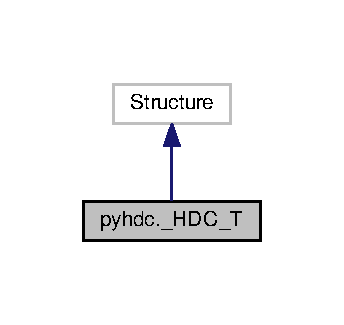
\includegraphics[width=165pt]{a00038}
\end{center}
\end{figure}


Collaboration diagram for pyhdc.\+\_\+\+H\+D\+C\+\_\+T\+:
\nopagebreak
\begin{figure}[H]
\begin{center}
\leavevmode
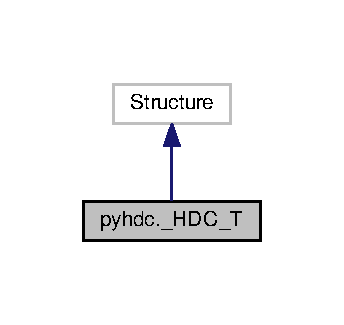
\includegraphics[width=165pt]{a00039}
\end{center}
\end{figure}


\subsection{Detailed Description}
\begin{DoxyVerb}HDC C pointer (opaque)
\end{DoxyVerb}
 

Definition at line 18 of file pyhdc.\+py.



The documentation for this class was generated from the following file\+:\begin{DoxyCompactItemize}
\item 
/home/david/projects/hdc\+\_\+new/src/pyhdc.\+py\end{DoxyCompactItemize}

\hypertarget{a00002}{}\section{pyhdc.\+H\+DC Class Reference}
\label{a00002}\index{pyhdc.\+H\+DC@{pyhdc.\+H\+DC}}


Inheritance diagram for pyhdc.\+H\+DC\+:
\nopagebreak
\begin{figure}[H]
\begin{center}
\leavevmode
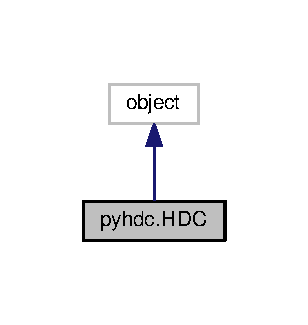
\includegraphics[width=148pt]{a00041}
\end{center}
\end{figure}


Collaboration diagram for pyhdc.\+H\+DC\+:
\nopagebreak
\begin{figure}[H]
\begin{center}
\leavevmode
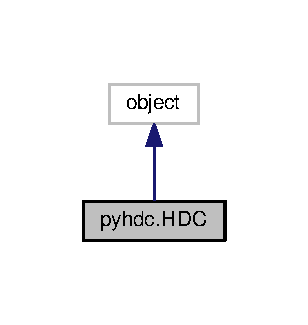
\includegraphics[width=148pt]{a00042}
\end{center}
\end{figure}
\subsection*{Public Member Functions}
\begin{DoxyCompactItemize}
\item 
def {\bfseries \+\_\+\+\_\+init\+\_\+\+\_\+} (self, data=None)\hypertarget{a00002_a2cad05f1fdef0f40c5bafacfd8345404}{}\label{a00002_a2cad05f1fdef0f40c5bafacfd8345404}

\item 
def {\bfseries from\+\_\+c\+\_\+ptr} (cls, c\+\_\+ptr)\hypertarget{a00002_adac78b1be622ccda340ff3d2bada6c80}{}\label{a00002_adac78b1be622ccda340ff3d2bada6c80}

\item 
def {\bfseries c\+\_\+ptr} (self)\hypertarget{a00002_a850482baa4f0fbb70d64d00ddb106d0b}{}\label{a00002_a850482baa4f0fbb70d64d00ddb106d0b}

\item 
def {\bfseries c\+\_\+ptr} (self, value)\hypertarget{a00002_a12837a146c289d28a0e3afb831fe095a}{}\label{a00002_a12837a146c289d28a0e3afb831fe095a}

\item 
def {\bfseries c\+\_\+ptr} (self, value)\hypertarget{a00002_a12837a146c289d28a0e3afb831fe095a}{}\label{a00002_a12837a146c289d28a0e3afb831fe095a}

\item 
def {\bfseries shape} (self)\hypertarget{a00002_a57ffc01d476e783c0f3cdc6e34b2acf5}{}\label{a00002_a57ffc01d476e783c0f3cdc6e34b2acf5}

\item 
def {\bfseries \+\_\+\+\_\+setitem\+\_\+\+\_\+} (self, key, value)\hypertarget{a00002_a50c2a3bcb7e6ed02394db3bcedbb90bd}{}\label{a00002_a50c2a3bcb7e6ed02394db3bcedbb90bd}

\item 
def {\bfseries \+\_\+\+\_\+getitem\+\_\+\+\_\+} (self, key)\hypertarget{a00002_a18c755c410c192bc9f944f54d03efcad}{}\label{a00002_a18c755c410c192bc9f944f54d03efcad}

\item 
def \hyperlink{a00002_a42b5d61d63e3ff6c9a0824eeaa5af88d}{set\+\_\+data} (self, data)
\item 
def {\bfseries get\+\_\+type\+\_\+str} (self)\hypertarget{a00002_a713e9156f96be1d70589536fe8466980}{}\label{a00002_a713e9156f96be1d70589536fe8466980}

\item 
def {\bfseries get\+\_\+shape} (self)\hypertarget{a00002_a2d338e04a2dac45cc0c14238236573d2}{}\label{a00002_a2d338e04a2dac45cc0c14238236573d2}

\item 
def {\bfseries tolist} (self)\hypertarget{a00002_a75eee53f2cdacdb2e6489d807781fb45}{}\label{a00002_a75eee53f2cdacdb2e6489d807781fb45}

\item 
def \hyperlink{a00002_a25c3660aa475054863838e9af3feae4b}{as\+\_\+array} (self)
\end{DoxyCompactItemize}
\subsection*{Public Attributes}
\begin{DoxyCompactItemize}
\item 
{\bfseries pydata}\hypertarget{a00002_a049aa20f1dc4d21c1df3ca7bde5d5194}{}\label{a00002_a049aa20f1dc4d21c1df3ca7bde5d5194}

\end{DoxyCompactItemize}


\subsection{Detailed Description}
\begin{DoxyVerb}HDC Python binding\end{DoxyVerb}
 

Definition at line 49 of file pyhdc.\+py.



\subsection{Member Function Documentation}
\index{pyhdc\+::\+H\+DC@{pyhdc\+::\+H\+DC}!as\+\_\+array@{as\+\_\+array}}
\index{as\+\_\+array@{as\+\_\+array}!pyhdc\+::\+H\+DC@{pyhdc\+::\+H\+DC}}
\subsubsection[{\texorpdfstring{as\+\_\+array(self)}{as_array(self)}}]{\setlength{\rightskip}{0pt plus 5cm}def pyhdc.\+H\+D\+C.\+as\+\_\+array (
\begin{DoxyParamCaption}
\item[{}]{self}
\end{DoxyParamCaption}
)}\hypertarget{a00002_a25c3660aa475054863838e9af3feae4b}{}\label{a00002_a25c3660aa475054863838e9af3feae4b}
\begin{DoxyVerb}Convert to a numpy array, sharing numerical data
\end{DoxyVerb}
 

Definition at line 145 of file pyhdc.\+py.


\begin{DoxyCode}
145     \textcolor{keyword}{def }\hyperlink{a00002_a25c3660aa475054863838e9af3feae4b}{as\_array}(self):
146         \textcolor{stringliteral}{"""Convert to a numpy array, sharing numerical data}
147 \textcolor{stringliteral}{        """}
148         type\_str = self.\hyperlink{a00002_a713e9156f96be1d70589536fe8466980}{get\_type\_str}()
149         \textcolor{keywordflow}{if} type\_str == \textcolor{stringliteral}{'hdc'}:
150             \textcolor{keywordflow}{return} np.array(self.\hyperlink{a00002_a75eee53f2cdacdb2e6489d807781fb45}{tolist}())
151         ctype = C\_TYPES\_MAP.get(type\_str, \textcolor{keywordtype}{None})
152         \textcolor{keywordflow}{if} ctype \textcolor{keywordflow}{is} \textcolor{keywordtype}{None}:
153             \textcolor{keywordflow}{raise} ValueError(\textcolor{stringliteral}{'Cannot convert \{\} to numpy array'}.format(type\_str))
154         c\_void\_ptr = \_hdc\_as\_voidptr(self.\hyperlink{a00002_ae96f30f5f5f55edcba46297da4e37d61}{\_c\_ptr})
155         cdata = ctypes.cast(c\_void\_ptr, ctype)
156         res = np.ctypeslib.as\_array(cdata, self.\hyperlink{a00002_a2d338e04a2dac45cc0c14238236573d2}{get\_shape}())
157 
158         \textcolor{keywordflow}{return} res
159 
160 
\end{DoxyCode}


Here is the call graph for this function\+:
\nopagebreak
\begin{figure}[H]
\begin{center}
\leavevmode
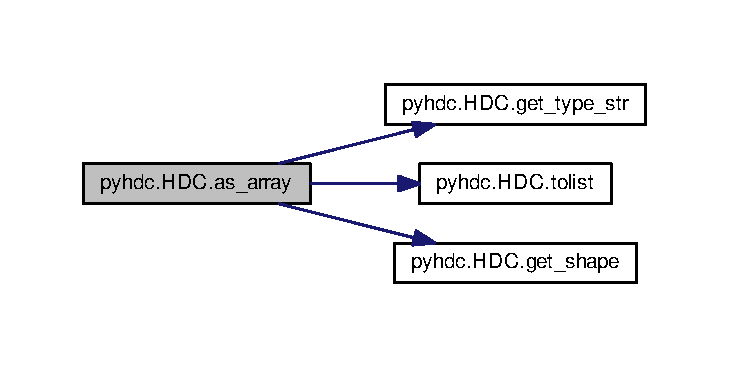
\includegraphics[width=350pt]{a00002_a25c3660aa475054863838e9af3feae4b_cgraph}
\end{center}
\end{figure}




Here is the caller graph for this function\+:
\nopagebreak
\begin{figure}[H]
\begin{center}
\leavevmode
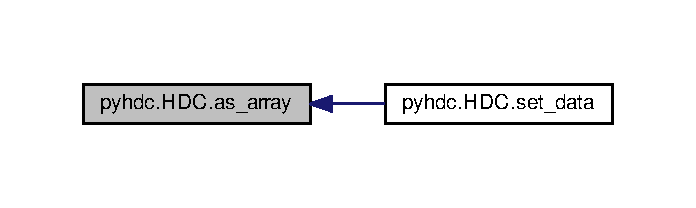
\includegraphics[width=334pt]{a00002_a25c3660aa475054863838e9af3feae4b_icgraph}
\end{center}
\end{figure}


\index{pyhdc\+::\+H\+DC@{pyhdc\+::\+H\+DC}!set\+\_\+data@{set\+\_\+data}}
\index{set\+\_\+data@{set\+\_\+data}!pyhdc\+::\+H\+DC@{pyhdc\+::\+H\+DC}}
\subsubsection[{\texorpdfstring{set\+\_\+data(self, data)}{set_data(self, data)}}]{\setlength{\rightskip}{0pt plus 5cm}def pyhdc.\+H\+D\+C.\+set\+\_\+data (
\begin{DoxyParamCaption}
\item[{}]{self, }
\item[{}]{data}
\end{DoxyParamCaption}
)}\hypertarget{a00002_a42b5d61d63e3ff6c9a0824eeaa5af88d}{}\label{a00002_a42b5d61d63e3ff6c9a0824eeaa5af88d}
\begin{DoxyVerb}Store data into the container
\end{DoxyVerb}
 

Definition at line 106 of file pyhdc.\+py.


\begin{DoxyCode}
106     \textcolor{keyword}{def }\hyperlink{a00002_a42b5d61d63e3ff6c9a0824eeaa5af88d}{set\_data}(self, data):
107         \textcolor{stringliteral}{"""Store data into the container}
108 \textcolor{stringliteral}{        """}
109         self.\hyperlink{a00002_a049aa20f1dc4d21c1df3ca7bde5d5194}{pydata} = data
110         \textcolor{keywordflow}{if} isinstance(data, np.ndarray):
111             \textcolor{comment}{# cdata = np.ctypeslib.as\_ctypes(data)}
112             cshape = np.ctypeslib.as\_ctypes(np.array(data.shape, dtype=np.int64))
113             cndim = ctypes.c\_int8(data.ndim)
114             \textcolor{keywordflow}{if} np.issubdtype(data.dtype, np.int8):
115                 cdata = data.ctypes.data\_as(ctypes.POINTER(ctypes.c\_int8))
116                 libchdc.hdc\_set\_data\_int8(self.\hyperlink{a00002_ae96f30f5f5f55edcba46297da4e37d61}{\_c\_ptr}, cndim, byref(cshape), cdata)
117             \textcolor{keywordflow}{elif} np.issubdtype(data.dtype, np.int32):
118                 cdata = data.ctypes.data\_as(ctypes.POINTER(ctypes.c\_int32))
119                 libchdc.hdc\_set\_data\_int32(self.\hyperlink{a00002_ae96f30f5f5f55edcba46297da4e37d61}{\_c\_ptr}, cndim, byref(cshape), cdata)
120             \textcolor{keywordflow}{elif} np.issubdtype(data.dtype, np.int64):
121                 cdata = data.ctypes.data\_as(ctypes.POINTER(ctypes.c\_int64))
122                 libchdc.hdc\_set\_data\_int64(self.\hyperlink{a00002_ae96f30f5f5f55edcba46297da4e37d61}{\_c\_ptr}, cndim, byref(cshape), cdata)
123             \textcolor{keywordflow}{elif} np.issubdtype(data.dtype, np.float\_):
124                 cdata = data.ctypes.data\_as(ctypes.POINTER(ctypes.c\_double))
125                 libchdc.hdc\_set\_data\_double(self.\hyperlink{a00002_ae96f30f5f5f55edcba46297da4e37d61}{\_c\_ptr}, cndim, byref(cshape), cdata)
126 
\end{DoxyCode}


Here is the call graph for this function\+:
\nopagebreak
\begin{figure}[H]
\begin{center}
\leavevmode
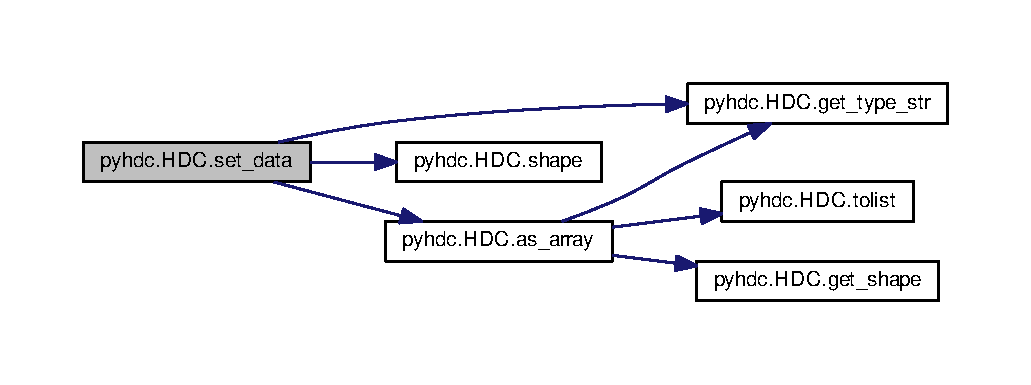
\includegraphics[width=350pt]{a00002_a42b5d61d63e3ff6c9a0824eeaa5af88d_cgraph}
\end{center}
\end{figure}




The documentation for this class was generated from the following file\+:\begin{DoxyCompactItemize}
\item 
/home/david/projects/hdc\+\_\+new/src/pyhdc.\+py\end{DoxyCompactItemize}

\hypertarget{a00003}{}\section{hdc Class Reference}
\label{a00003}\index{hdc@{hdc}}
\subsection*{Public Member Functions}
\begin{DoxyCompactItemize}
\item 
\hyperlink{a00003_a0dd2786f4236f02ac3c5895a9f9dc0fd}{hdc} (dynd\+::nd\+::array arr)
\begin{DoxyCompactList}\small\item\em Default constructor. \end{DoxyCompactList}\item 
\hyperlink{a00003_a18f8ee62caf1d5ae22d65d9dd330f9cc}{$\sim$hdc} ()
\begin{DoxyCompactList}\small\item\em Creates H\+DC with data from Dy\+ND array object. \end{DoxyCompactList}\item 
void \hyperlink{a00003_a6ae2658ee66a5f4fb0d0d6535b36c5b2}{add\+\_\+child} (string path, \hyperlink{a00003}{hdc} $\ast$n)\hypertarget{a00003_a6ae2658ee66a5f4fb0d0d6535b36c5b2}{}\label{a00003_a6ae2658ee66a5f4fb0d0d6535b36c5b2}

\begin{DoxyCompactList}\small\item\em Desctructor. \end{DoxyCompactList}\item 
void \hyperlink{a00003_acde60e58222d3b7d2b2a53b14289f500}{set\+\_\+child} (string path, \hyperlink{a00003}{hdc} $\ast$n)
\begin{DoxyCompactList}\small\item\em Adds H\+DC subtree as child with given path. \end{DoxyCompactList}\item 
void \hyperlink{a00003_af2b7f95b9cf36d26e0fc20dd1c0465ba}{delete\+\_\+child} (string path)
\begin{DoxyCompactList}\small\item\em Sets H\+DC subtree to given path. \end{DoxyCompactList}\item 
\hyperlink{a00003}{hdc} $\ast$ \hyperlink{a00003_aafcd7c001cf4d3e2d61dbbf6efef6e08}{get\+\_\+child} (string path)
\begin{DoxyCompactList}\small\item\em Deletes H\+DC subtree. \end{DoxyCompactList}\item 
\hyperlink{a00003}{hdc} $\ast$ \hyperlink{a00003_a580b1c84ebb50da63e2682ddceb6010a}{get\+\_\+slice} (string path, size\+\_\+t i)
\begin{DoxyCompactList}\small\item\em Returns subtree by path. \end{DoxyCompactList}\item 
\hyperlink{a00003}{hdc} $\ast$ \hyperlink{a00003_a1ef96265e222ef9acc07c151b20af8bf}{get\+\_\+slice} (size\+\_\+t i)
\begin{DoxyCompactList}\small\item\em Returns i-\/th subnode if H\+D\+C\+\_\+\+L\+I\+ST is the type. \end{DoxyCompactList}\item 
bool \hyperlink{a00003_aee70cadad065fa643d8313e068734e59}{has\+\_\+child} (string path)
\begin{DoxyCompactList}\small\item\em Returns i-\/th subnode if H\+D\+C\+\_\+\+L\+I\+ST is the type. \end{DoxyCompactList}\item 
{\footnotesize template$<$typename T $>$ }\\void \hyperlink{a00003_a120de413f9264db573e7c54aa49ae489}{set\+\_\+data} (vector$<$ T $>$ data)
\begin{DoxyCompactList}\small\item\em Returns true if subtree with given path with exists and false otherwise. \end{DoxyCompactList}\item 
{\footnotesize template$<$typename T $>$ }\\void \hyperlink{a00003_a9462ce2e878c8e978e38a9f71188973b}{set\+\_\+data} (string path, vector$<$ T $>$ data)
\begin{DoxyCompactList}\small\item\em Sets data to node on given path from vector$<$\+T$>$ data. \end{DoxyCompactList}\item 
{\footnotesize template$<$typename T $>$ }\\void \hyperlink{a00003_a42e2debec93119c4e79ddefb49ff5c43}{set\+\_\+data} (int8\+\_\+t ndim, const long int $\ast$shape, void $\ast$data)
\begin{DoxyCompactList}\small\item\em Sets array data to current node. \end{DoxyCompactList}\item 
{\footnotesize template$<$typename T $>$ }\\void \hyperlink{a00003_a009b92dac161a40dc8e17231a4575c1a}{set\+\_\+data} (string path, int8\+\_\+t ndim, const long int $\ast$shape, void $\ast$data)
\begin{DoxyCompactList}\small\item\em Sets array data to node on given path. \end{DoxyCompactList}\item 
{\footnotesize template$<$typename T $>$ }\\void \hyperlink{a00003_a4465da11f7821ef4d405cd8805d77459}{set\+\_\+data} (T data)
\begin{DoxyCompactList}\small\item\em Sets scalar data to current node. \end{DoxyCompactList}\item 
{\footnotesize template$<$typename T $>$ }\\void \hyperlink{a00003_a5a15d6128e566f802263c3fbf69a1d49}{set\+\_\+data} (string path, T data)
\begin{DoxyCompactList}\small\item\em Sets scalar data to node on given path. \end{DoxyCompactList}\item 
void {\bfseries set\+\_\+dynd} (dynd\+::nd\+::array array)\hypertarget{a00003_a4fae038574f9adbc8b6dbb8524677097}{}\label{a00003_a4fae038574f9adbc8b6dbb8524677097}

\item 
void \hyperlink{a00003_ae3cf31bad48437a48ad1291e2db99873}{set\+\_\+list} (vector$<$ \hyperlink{a00003}{hdc} $\ast$ $>$ $\ast$list)
\begin{DoxyCompactList}\small\item\em Sets Dy\+ND object to current node. \end{DoxyCompactList}\item 
void \hyperlink{a00003_ab88feab4710f598b8a56b529fd01dede}{create\+\_\+list} (size\+\_\+t n=5)
\begin{DoxyCompactList}\small\item\em Sets D\+H\+C\+\_\+\+L\+I\+ST from std\+::vector$<$hdc$\ast$$>$ data. \end{DoxyCompactList}\item 
void \hyperlink{a00003_ad782f111cf0c869166ed9f4ac51405a6}{resize} (\hyperlink{a00003}{hdc} $\ast$h, int recursively=0)
\begin{DoxyCompactList}\small\item\em Creates list with some data in nodes -\/ just for testing some ideas. \end{DoxyCompactList}\item 
\hyperlink{a00003}{hdc} $\ast$ \hyperlink{a00003_af5d54732a2d9d34f7f2f8453acda21d6}{copy} (int copy\+\_\+arrays=0)
\begin{DoxyCompactList}\small\item\em Performs deep copy of current node if recursively = 1. \end{DoxyCompactList}\item 
void \hyperlink{a00003_a3d4c2ba09c79e2dfbe7be7bd59bd811e}{set\+\_\+slice} (size\+\_\+t i, \hyperlink{a00003}{hdc} $\ast$h)
\begin{DoxyCompactList}\small\item\em Returns copy of current object. \end{DoxyCompactList}\item 
void \hyperlink{a00003_aaffff0cd041746fd45a2d2c67d73ce75}{append\+\_\+slice} (\hyperlink{a00003}{hdc} $\ast$h)
\begin{DoxyCompactList}\small\item\em Sets node to i-\/th slice of current node. \end{DoxyCompactList}\item 
uint8\+\_\+t \hyperlink{a00003_ac12e6d9074533304ea4d3eb08623d774}{get\+\_\+type} ()
\begin{DoxyCompactList}\small\item\em Appends given node as next available slice (similar to push\+\_\+back() method seen in C++ S\+TL containers). \end{DoxyCompactList}\item 
void \hyperlink{a00003_a6d1d1064db92be176775481eb6ca9fd3}{set\+\_\+type} (uint8\+\_\+t i)
\begin{DoxyCompactList}\small\item\em Returns type of current node. \end{DoxyCompactList}\item 
bool \hyperlink{a00003_af1a86c27a06e02651f544947eb9b0cfb}{is\+\_\+empty} ()
\begin{DoxyCompactList}\small\item\em Sets H\+DC type of current node. \end{DoxyCompactList}\item 
int8\+\_\+t \hyperlink{a00003_a759758dd2b6b8986341753e94ad12252}{get\+\_\+ndim} ()
\begin{DoxyCompactList}\small\item\em Returns true if node is empty. \end{DoxyCompactList}\item 
long int $\ast$ \hyperlink{a00003_aa73e21aec9037f1f6bf9bb899f743b00}{get\+\_\+shape} ()
\begin{DoxyCompactList}\small\item\em Returns number of dimensions of current node. \end{DoxyCompactList}\item 
int8\+\_\+t \hyperlink{a00003_ac8d2e3eb577519c8caa5ea59a34ae75b}{get\+\_\+ndim} (string path)
\begin{DoxyCompactList}\small\item\em Shape of array. \end{DoxyCompactList}\item 
long int $\ast$ \hyperlink{a00003_a9684ce622a000411e1c747f4f694c92f}{get\+\_\+shape} (string path)
\begin{DoxyCompactList}\small\item\em Returns number of dimensions of node under path. \end{DoxyCompactList}\item 
{\footnotesize template$<$typename T $>$ }\\T \hyperlink{a00003_ae35cce784c60574515001b66d0271fa9}{as} ()
\begin{DoxyCompactList}\small\item\em Returns shape of node under path. \end{DoxyCompactList}\item 
{\footnotesize template$<$typename T $>$ }\\T \hyperlink{a00003_ac1dd72a041586072f7984022ba8a048e}{as} (string path)
\begin{DoxyCompactList}\small\item\em Returns pointer to data of node under given path. \end{DoxyCompactList}\item 
double \hyperlink{a00003_a12e3492b3755543da2c6b1571629e23c}{as\+\_\+double} ()
\begin{DoxyCompactList}\small\item\em Returns double. \end{DoxyCompactList}\item 
double \hyperlink{a00003_a10b21a25e3429e9844084b74a8bacbaa}{as\+\_\+double} (string path)
\begin{DoxyCompactList}\small\item\em Returns double. \end{DoxyCompactList}\item 
\hyperlink{a00007}{hdc\+\_\+t} $\ast$ {\bfseries as\+\_\+hdc\+\_\+ptr} ()\hypertarget{a00003_aea48e6e093255899e87151031408d0eb}{}\label{a00003_aea48e6e093255899e87151031408d0eb}

\item 
void \hyperlink{a00003_af7684e94ec717ae6e9de1ba1f0e6bff0}{to\+\_\+json} (string filename, int mode=0)
\begin{DoxyCompactList}\small\item\em Returns pointer to self. \end{DoxyCompactList}\item 
Json\+::\+Value \hyperlink{a00003_a801f7f1bd6c145b0fef673b99b0724d2}{to\+\_\+json} (int mode=0)
\begin{DoxyCompactList}\small\item\em Serialization to J\+S\+ON file. \end{DoxyCompactList}\item 
void $\ast$ \hyperlink{a00003_ae3c66b7860c6394eb777770d0601fceb}{as\+\_\+void\+\_\+ptr} ()
\begin{DoxyCompactList}\small\item\em Serialization to Json\+::\+Value object. \end{DoxyCompactList}\item 
string \hyperlink{a00003_adb9061053ac1426deae825e364b340bc}{get\+\_\+type\+\_\+str} ()
\begin{DoxyCompactList}\small\item\em Returns void pointer to data. \end{DoxyCompactList}\item 
string \hyperlink{a00003_a57618e790b5eb42e4fb3f35fe95eed07}{get\+\_\+datashape\+\_\+str} ()
\begin{DoxyCompactList}\small\item\em Returns string representing data/node type. \end{DoxyCompactList}\end{DoxyCompactItemize}


\subsection{Detailed Description}


Definition at line 34 of file hdc.\+hpp.



\subsection{Constructor \& Destructor Documentation}
\index{hdc@{hdc}!hdc@{hdc}}
\index{hdc@{hdc}!hdc@{hdc}}
\subsubsection[{\texorpdfstring{hdc(dynd\+::nd\+::array arr)}{hdc(dynd::nd::array arr)}}]{\setlength{\rightskip}{0pt plus 5cm}hdc\+::hdc (
\begin{DoxyParamCaption}
\item[{dynd\+::nd\+::array}]{arr}
\end{DoxyParamCaption}
)}\hypertarget{a00003_a0dd2786f4236f02ac3c5895a9f9dc0fd}{}\label{a00003_a0dd2786f4236f02ac3c5895a9f9dc0fd}


Default constructor. 

Creates empty H\+DC 

Definition at line 24 of file hdc.\+cpp.


\begin{DoxyCode}
24                         \{
25     cout << \textcolor{stringliteral}{"Creating DyND node..."} << endl;
26     type = HDC\_DYND;
27     data = \textcolor{keyword}{new} vector<dynd::nd::array>;
28     children = \textcolor{keyword}{new} unordered\_map<string, hdc*>;
29     list\_elements = \textcolor{keyword}{nullptr};
30     data->push\_back(arr);
31 \}
\end{DoxyCode}
\index{hdc@{hdc}!````~hdc@{$\sim$hdc}}
\index{````~hdc@{$\sim$hdc}!hdc@{hdc}}
\subsubsection[{\texorpdfstring{$\sim$hdc()}{~hdc()}}]{\setlength{\rightskip}{0pt plus 5cm}hdc\+::$\sim$hdc (
\begin{DoxyParamCaption}
{}
\end{DoxyParamCaption}
)}\hypertarget{a00003_a18f8ee62caf1d5ae22d65d9dd330f9cc}{}\label{a00003_a18f8ee62caf1d5ae22d65d9dd330f9cc}


Creates H\+DC with data from Dy\+ND array object. 



Definition at line 33 of file hdc.\+cpp.


\begin{DoxyCode}
34 \{
35     cout << \textcolor{stringliteral}{"Destructor called..."} << endl;
36     \textcolor{keywordflow}{if} (!children->empty()) \{
37         cout << \textcolor{stringliteral}{"Deleting children..."} << endl;
38         \textcolor{keywordflow}{for} (\textcolor{keyword}{auto} it = children->begin(); it != children->end(); it++) \textcolor{keyword}{delete} it->second;
39         children->clear();
40     \} \textcolor{keywordflow}{else} \{
41         \textcolor{keyword}{delete} children;
42         \textcolor{keyword}{delete} data;
43         \textcolor{keywordflow}{if} (list\_elements != \textcolor{keyword}{nullptr}) \{
44             \textcolor{keywordflow}{for} (\textcolor{keywordtype}{size\_t} i;i < list\_elements->size();i++) \textcolor{keyword}{delete} &list\_elements[i];
45             list\_elements->clear();
46             \textcolor{keyword}{delete} list\_elements;
47         \}
48     \}
49 \}
\end{DoxyCode}


\subsection{Member Function Documentation}
\index{hdc@{hdc}!append\+\_\+slice@{append\+\_\+slice}}
\index{append\+\_\+slice@{append\+\_\+slice}!hdc@{hdc}}
\subsubsection[{\texorpdfstring{append\+\_\+slice(hdc $\ast$h)}{append_slice(hdc *h)}}]{\setlength{\rightskip}{0pt plus 5cm}void hdc\+::append\+\_\+slice (
\begin{DoxyParamCaption}
\item[{{\bf hdc} $\ast$}]{h}
\end{DoxyParamCaption}
)}\hypertarget{a00003_aaffff0cd041746fd45a2d2c67d73ce75}{}\label{a00003_aaffff0cd041746fd45a2d2c67d73ce75}


Sets node to i-\/th slice of current node. 



Definition at line 489 of file hdc.\+cpp.


\begin{DoxyCode}
489                              \{
490     \textcolor{keywordflow}{if} (this->type == HDC\_EMPTY) \{
491         this->\hyperlink{a00003_a6d1d1064db92be176775481eb6ca9fd3}{set\_type}(HDC\_LIST);
492     \}
493     \textcolor{keywordflow}{if} (this->type == HDC\_LIST) \{
494         this->list\_elements->push\_back(h);
495     \} \textcolor{keywordflow}{else} \{
496         cout << \textcolor{stringliteral}{"Error: append\_slice not supported for HDC\_STRUCT"} << endl;
497         exit(-1);
498     \}
499     \textcolor{keywordflow}{return};
500 \}
\end{DoxyCode}


Here is the caller graph for this function\+:
\nopagebreak
\begin{figure}[H]
\begin{center}
\leavevmode
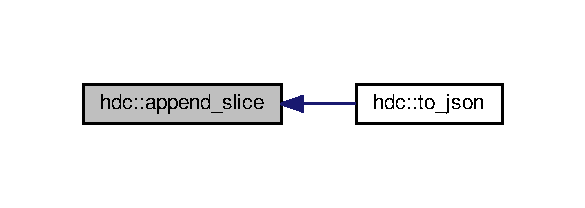
\includegraphics[width=281pt]{a00003_aaffff0cd041746fd45a2d2c67d73ce75_icgraph}
\end{center}
\end{figure}


\index{hdc@{hdc}!as@{as}}
\index{as@{as}!hdc@{hdc}}
\subsubsection[{\texorpdfstring{as()}{as()}}]{\setlength{\rightskip}{0pt plus 5cm}template$<$typename T $>$ T hdc\+::as (
\begin{DoxyParamCaption}
{}
\end{DoxyParamCaption}
)\hspace{0.3cm}{\ttfamily [inline]}}\hypertarget{a00003_ae35cce784c60574515001b66d0271fa9}{}\label{a00003_ae35cce784c60574515001b66d0271fa9}


Returns shape of node under path. 

Returns pointer to data of this node. 

Definition at line 144 of file hdc.\+hpp.


\begin{DoxyCode}
145     \{
146         \textcolor{comment}{// returns data of given type}
147         \textcolor{keywordflow}{if} (this->children->size()) \{
148             cout << \textcolor{stringliteral}{"This node is not terminal"} << endl;
149         \}
150         cout << \textcolor{stringliteral}{"From get:"} << this->data->at(0) << endl;
151 \textcolor{comment}{//         return (T)(this->data->at(0)->data);}
152         \textcolor{keywordflow}{return} (T)(this->data->at(0).get());
153         
154         \textcolor{comment}{//return (T)(this->data.data());}
155     \}
\end{DoxyCode}


Here is the caller graph for this function\+:
\nopagebreak
\begin{figure}[H]
\begin{center}
\leavevmode
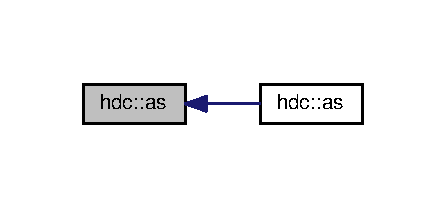
\includegraphics[width=214pt]{a00003_ae35cce784c60574515001b66d0271fa9_icgraph}
\end{center}
\end{figure}


\index{hdc@{hdc}!as@{as}}
\index{as@{as}!hdc@{hdc}}
\subsubsection[{\texorpdfstring{as(string path)}{as(string path)}}]{\setlength{\rightskip}{0pt plus 5cm}template$<$typename T $>$ T hdc\+::as (
\begin{DoxyParamCaption}
\item[{string}]{path}
\end{DoxyParamCaption}
)\hspace{0.3cm}{\ttfamily [inline]}}\hypertarget{a00003_ac1dd72a041586072f7984022ba8a048e}{}\label{a00003_ac1dd72a041586072f7984022ba8a048e}


Returns pointer to data of node under given path. 



Definition at line 157 of file hdc.\+hpp.


\begin{DoxyCode}
158     \{
159         cout << \textcolor{stringliteral}{"as<T>("} << path << \textcolor{stringliteral}{")"} << endl;
160         \textcolor{comment}{// returns data of given type}
161         \hyperlink{a00003}{hdc}* t = this->\hyperlink{a00003_aafcd7c001cf4d3e2d61dbbf6efef6e08}{get\_child}(path);
162         \textcolor{keywordflow}{return} t->\hyperlink{a00003_ae35cce784c60574515001b66d0271fa9}{as}<T>();
163     \}
\end{DoxyCode}


Here is the call graph for this function\+:
\nopagebreak
\begin{figure}[H]
\begin{center}
\leavevmode
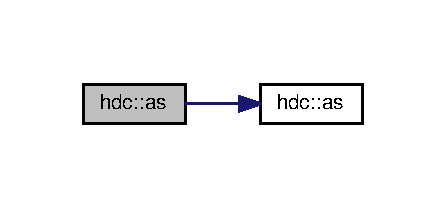
\includegraphics[width=214pt]{a00003_ac1dd72a041586072f7984022ba8a048e_cgraph}
\end{center}
\end{figure}


\index{hdc@{hdc}!as\+\_\+double@{as\+\_\+double}}
\index{as\+\_\+double@{as\+\_\+double}!hdc@{hdc}}
\subsubsection[{\texorpdfstring{as\+\_\+double()}{as_double()}}]{\setlength{\rightskip}{0pt plus 5cm}double hdc\+::as\+\_\+double (
\begin{DoxyParamCaption}
{}
\end{DoxyParamCaption}
)\hspace{0.3cm}{\ttfamily [inline]}}\hypertarget{a00003_a12e3492b3755543da2c6b1571629e23c}{}\label{a00003_a12e3492b3755543da2c6b1571629e23c}


Returns double. 



Definition at line 164 of file hdc.\+hpp.


\begin{DoxyCode}
165     \{
166         \textcolor{keywordflow}{return} this->as<double*>()[0];
167     \}
\end{DoxyCode}
\index{hdc@{hdc}!as\+\_\+double@{as\+\_\+double}}
\index{as\+\_\+double@{as\+\_\+double}!hdc@{hdc}}
\subsubsection[{\texorpdfstring{as\+\_\+double(string path)}{as_double(string path)}}]{\setlength{\rightskip}{0pt plus 5cm}double hdc\+::as\+\_\+double (
\begin{DoxyParamCaption}
\item[{string}]{path}
\end{DoxyParamCaption}
)\hspace{0.3cm}{\ttfamily [inline]}}\hypertarget{a00003_a10b21a25e3429e9844084b74a8bacbaa}{}\label{a00003_a10b21a25e3429e9844084b74a8bacbaa}


Returns double. 



Definition at line 168 of file hdc.\+hpp.


\begin{DoxyCode}
169     \{
170         \textcolor{keywordflow}{return} this->as<double*>(path)[0];
171     \}
\end{DoxyCode}
\index{hdc@{hdc}!as\+\_\+void\+\_\+ptr@{as\+\_\+void\+\_\+ptr}}
\index{as\+\_\+void\+\_\+ptr@{as\+\_\+void\+\_\+ptr}!hdc@{hdc}}
\subsubsection[{\texorpdfstring{as\+\_\+void\+\_\+ptr()}{as_void_ptr()}}]{\setlength{\rightskip}{0pt plus 5cm}void $\ast$ hdc\+::as\+\_\+void\+\_\+ptr (
\begin{DoxyParamCaption}
{}
\end{DoxyParamCaption}
)}\hypertarget{a00003_ae3c66b7860c6394eb777770d0601fceb}{}\label{a00003_ae3c66b7860c6394eb777770d0601fceb}


Serialization to Json\+::\+Value object. 



Definition at line 276 of file hdc.\+cpp.


\begin{DoxyCode}
276                        \{
277     \textcolor{keywordflow}{return} (\textcolor{keywordtype}{void}*)\textcolor{keyword}{this};
278 \}
\end{DoxyCode}
\index{hdc@{hdc}!copy@{copy}}
\index{copy@{copy}!hdc@{hdc}}
\subsubsection[{\texorpdfstring{copy(int copy\+\_\+arrays=0)}{copy(int copy_arrays=0)}}]{\setlength{\rightskip}{0pt plus 5cm}{\bf hdc} $\ast$ hdc\+::copy (
\begin{DoxyParamCaption}
\item[{int}]{copy\+\_\+arrays = {\ttfamily 0}}
\end{DoxyParamCaption}
)}\hypertarget{a00003_af5d54732a2d9d34f7f2f8453acda21d6}{}\label{a00003_af5d54732a2d9d34f7f2f8453acda21d6}


Performs deep copy of current node if recursively = 1. 

Performs shallow copy otherwise. 

Definition at line 450 of file hdc.\+cpp.


\begin{DoxyCode}
451 \{
452     cout << \textcolor{stringliteral}{"Called copy()"} << endl;
453     \hyperlink{a00003}{hdc}* \hyperlink{a00003_af5d54732a2d9d34f7f2f8453acda21d6}{copy} = \textcolor{keyword}{new} \hyperlink{a00003}{hdc}();
454     copy->\hyperlink{a00003_a6d1d1064db92be176775481eb6ca9fd3}{set\_type}(this->\hyperlink{a00003_ac12e6d9074533304ea4d3eb08623d774}{get\_type}());
455     cout << (int)(this->\hyperlink{a00003_ac12e6d9074533304ea4d3eb08623d774}{get\_type}()) << endl;
456     \textcolor{keywordflow}{if} (this->type == HDC\_STRUCT) \{
457         \textcolor{keywordflow}{for} (\textcolor{keyword}{auto} it = this->children->begin(); it != this->children->end(); it++) \{
458             copy->\hyperlink{a00003_a6ae2658ee66a5f4fb0d0d6535b36c5b2}{add\_child}(it->first,it->second->copy(copy\_arrays));
459             cout << it->first << \textcolor{stringliteral}{" copied"} << endl;
460         \}
461     \} \textcolor{keywordflow}{else} \textcolor{keywordflow}{if} (this->type == HDC\_LIST) \{
462         \textcolor{keywordflow}{for} (\textcolor{keywordtype}{size\_t} i = 0; i < this->list\_elements->size(); i++)
463             copy->\hyperlink{a00003_a3d4c2ba09c79e2dfbe7be7bd59bd811e}{set\_slice}(i,this->list\_elements->at(i)->copy(copy\_arrays));
464     \}
465     \textcolor{keywordflow}{else} \textcolor{keywordflow}{if} (this->type == HDC\_DYND) \{
466         \textcolor{keywordflow}{if} (copy\_arrays == 1) \{
467             \textcolor{comment}{//dynd::nd::empty(<this->data->at(0).get\_type()>);}
468             \textcolor{comment}{//long size = this->data->at(0).size();}
469             \textcolor{comment}{//char *}
470             copy->data->push\_back(dynd::nd::array(this->data->at(0)));
471             cout << \textcolor{stringliteral}{"copy: "} << copy->data->at(0) << endl;
472         \} \textcolor{keywordflow}{else} this->\hyperlink{a00003_a6d1d1064db92be176775481eb6ca9fd3}{set\_type}(HDC\_EMPTY);
473     \}
474     cout << \textcolor{stringliteral}{"copy() Done"} << endl;
475     \textcolor{keywordflow}{return} \hyperlink{a00003_af5d54732a2d9d34f7f2f8453acda21d6}{copy};
476 \}
\end{DoxyCode}


Here is the call graph for this function\+:
\nopagebreak
\begin{figure}[H]
\begin{center}
\leavevmode
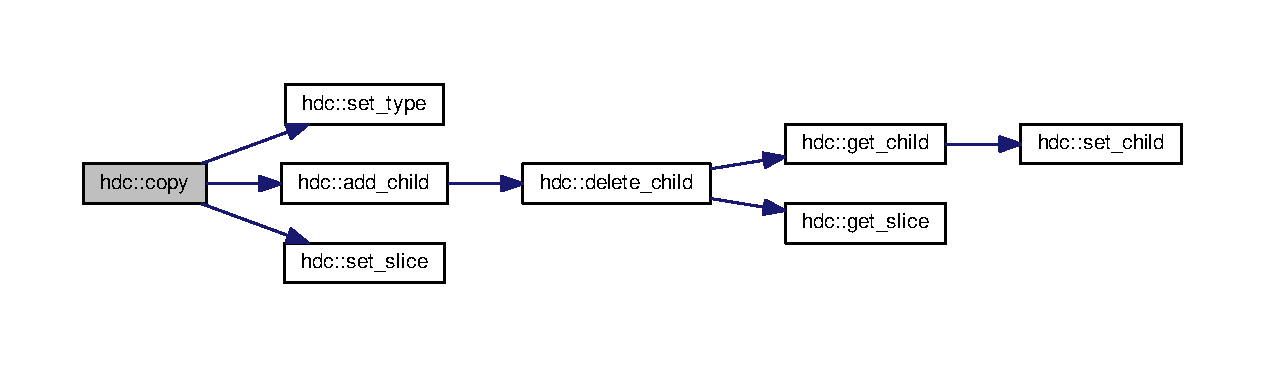
\includegraphics[width=350pt]{a00003_af5d54732a2d9d34f7f2f8453acda21d6_cgraph}
\end{center}
\end{figure}


\index{hdc@{hdc}!create\+\_\+list@{create\+\_\+list}}
\index{create\+\_\+list@{create\+\_\+list}!hdc@{hdc}}
\subsubsection[{\texorpdfstring{create\+\_\+list(size\+\_\+t n=5)}{create_list(size_t n=5)}}]{\setlength{\rightskip}{0pt plus 5cm}void hdc\+::create\+\_\+list (
\begin{DoxyParamCaption}
\item[{size\+\_\+t}]{n = {\ttfamily 5}}
\end{DoxyParamCaption}
)}\hypertarget{a00003_ab88feab4710f598b8a56b529fd01dede}{}\label{a00003_ab88feab4710f598b8a56b529fd01dede}


Sets D\+H\+C\+\_\+\+L\+I\+ST from std\+::vector$<$hdc$\ast$$>$ data. 



Definition at line 115 of file hdc.\+cpp.


\begin{DoxyCode}
115                               \{
116     \textcolor{keywordflow}{if} (this->type != HDC\_EMPTY) \{
117         cout << \textcolor{stringliteral}{"Cannot add list to a non-list node."} << endl;
118     \}
119     this->type = HDC\_LIST;
120     this->list\_elements = \textcolor{keyword}{new} vector<hdc*>;
121     \textcolor{keywordflow}{for} (\textcolor{keywordtype}{size\_t} i=0; i<n;i++) list\_elements->push\_back(\textcolor{keyword}{new} \hyperlink{a00003}{hdc}());
122     \textcolor{comment}{//debuging}
123     \textcolor{keywordflow}{for} (\textcolor{keywordtype}{size\_t} i=0; i<n;i++) \{
124         int8\_t* arr = \textcolor{keyword}{new} int8\_t[1];
125         arr[0] = i;
126         \textcolor{keywordtype}{long} shape[] = \{1\};
127         list\_elements->at(i)->set\_data<int8\_t>(1,(\textcolor{keywordtype}{long} \textcolor{keywordtype}{int}*)shape,(\textcolor{keywordtype}{void}*)arr);    
128     \}
129     return;
130 \}
\end{DoxyCode}
\index{hdc@{hdc}!delete\+\_\+child@{delete\+\_\+child}}
\index{delete\+\_\+child@{delete\+\_\+child}!hdc@{hdc}}
\subsubsection[{\texorpdfstring{delete\+\_\+child(string path)}{delete_child(string path)}}]{\setlength{\rightskip}{0pt plus 5cm}void hdc\+::delete\+\_\+child (
\begin{DoxyParamCaption}
\item[{string}]{path}
\end{DoxyParamCaption}
)}\hypertarget{a00003_af2b7f95b9cf36d26e0fc20dd1c0465ba}{}\label{a00003_af2b7f95b9cf36d26e0fc20dd1c0465ba}


Sets H\+DC subtree to given path. 



Definition at line 159 of file hdc.\+cpp.


\begin{DoxyCode}
159                                   \{
160     this->\hyperlink{a00003_af2b7f95b9cf36d26e0fc20dd1c0465ba}{delete\_child}(split(path,\textcolor{charliteral}{'/'}));
161     \textcolor{keywordflow}{return};
162 \}
\end{DoxyCode}


Here is the call graph for this function\+:
\nopagebreak
\begin{figure}[H]
\begin{center}
\leavevmode
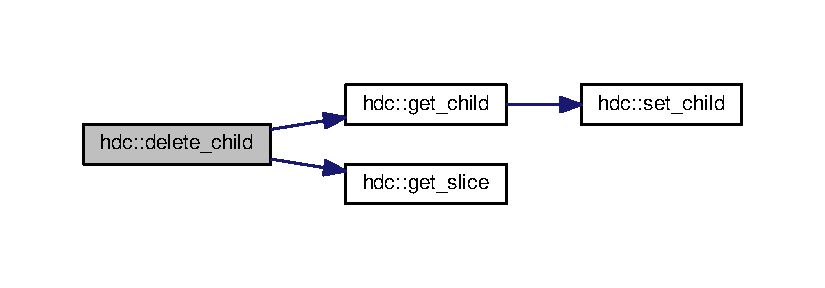
\includegraphics[width=350pt]{a00003_af2b7f95b9cf36d26e0fc20dd1c0465ba_cgraph}
\end{center}
\end{figure}




Here is the caller graph for this function\+:
\nopagebreak
\begin{figure}[H]
\begin{center}
\leavevmode
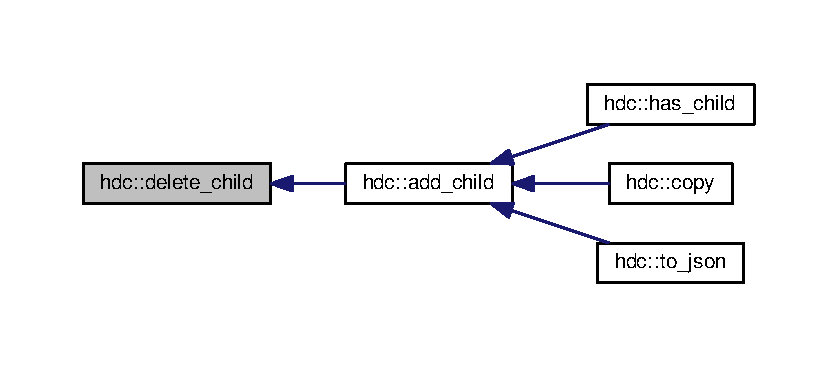
\includegraphics[width=350pt]{a00003_af2b7f95b9cf36d26e0fc20dd1c0465ba_icgraph}
\end{center}
\end{figure}


\index{hdc@{hdc}!get\+\_\+child@{get\+\_\+child}}
\index{get\+\_\+child@{get\+\_\+child}!hdc@{hdc}}
\subsubsection[{\texorpdfstring{get\+\_\+child(string path)}{get_child(string path)}}]{\setlength{\rightskip}{0pt plus 5cm}{\bf hdc} $\ast$ hdc\+::get\+\_\+child (
\begin{DoxyParamCaption}
\item[{string}]{path}
\end{DoxyParamCaption}
)}\hypertarget{a00003_aafcd7c001cf4d3e2d61dbbf6efef6e08}{}\label{a00003_aafcd7c001cf4d3e2d61dbbf6efef6e08}


Deletes H\+DC subtree. 



Definition at line 217 of file hdc.\+cpp.


\begin{DoxyCode}
217                                \{
218     \textcolor{keywordflow}{return} this->\hyperlink{a00003_aafcd7c001cf4d3e2d61dbbf6efef6e08}{get\_child}(split(path,\textcolor{charliteral}{'/'}));
219 \}
\end{DoxyCode}


Here is the call graph for this function\+:
\nopagebreak
\begin{figure}[H]
\begin{center}
\leavevmode
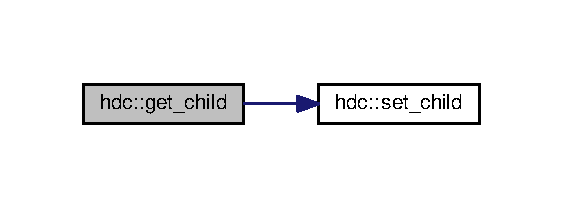
\includegraphics[width=270pt]{a00003_aafcd7c001cf4d3e2d61dbbf6efef6e08_cgraph}
\end{center}
\end{figure}




Here is the caller graph for this function\+:
\nopagebreak
\begin{figure}[H]
\begin{center}
\leavevmode
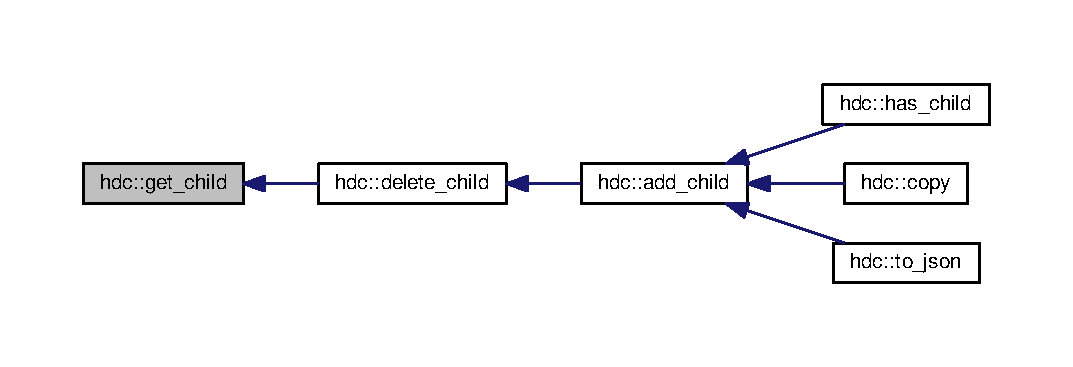
\includegraphics[width=350pt]{a00003_aafcd7c001cf4d3e2d61dbbf6efef6e08_icgraph}
\end{center}
\end{figure}


\index{hdc@{hdc}!get\+\_\+datashape\+\_\+str@{get\+\_\+datashape\+\_\+str}}
\index{get\+\_\+datashape\+\_\+str@{get\+\_\+datashape\+\_\+str}!hdc@{hdc}}
\subsubsection[{\texorpdfstring{get\+\_\+datashape\+\_\+str()}{get_datashape_str()}}]{\setlength{\rightskip}{0pt plus 5cm}string hdc\+::get\+\_\+datashape\+\_\+str (
\begin{DoxyParamCaption}
{}
\end{DoxyParamCaption}
)}\hypertarget{a00003_a57618e790b5eb42e4fb3f35fe95eed07}{}\label{a00003_a57618e790b5eb42e4fb3f35fe95eed07}


Returns string representing data/node type. 



Definition at line 543 of file hdc.\+cpp.


\begin{DoxyCode}
543                               \{
544     \textcolor{keywordtype}{string} type\_str;
545     \textcolor{keywordflow}{if} (this->type == HDC\_EMPTY) type\_str = \textcolor{stringliteral}{"null"};
546     \textcolor{keywordflow}{else} \textcolor{keywordflow}{if} (this->type == HDC\_LIST || this->type == HDC\_STRUCT) type\_str = \textcolor{stringliteral}{"hdc"};
547     \textcolor{keywordflow}{else} \{
548         dynd::ndt::type dt;
549         dt = this->data->at(0).get\_type();
550         type\_str = dt.str();
551     \}
552     \textcolor{keywordflow}{return} type\_str;
553 \}
\end{DoxyCode}
\index{hdc@{hdc}!get\+\_\+ndim@{get\+\_\+ndim}}
\index{get\+\_\+ndim@{get\+\_\+ndim}!hdc@{hdc}}
\subsubsection[{\texorpdfstring{get\+\_\+ndim()}{get_ndim()}}]{\setlength{\rightskip}{0pt plus 5cm}int8\+\_\+t hdc\+::get\+\_\+ndim (
\begin{DoxyParamCaption}
{}
\end{DoxyParamCaption}
)}\hypertarget{a00003_a759758dd2b6b8986341753e94ad12252}{}\label{a00003_a759758dd2b6b8986341753e94ad12252}


Returns true if node is empty. 



Definition at line 265 of file hdc.\+cpp.


\begin{DoxyCode}
266 \{
267     \textcolor{keywordflow}{if} (this->type == HDC\_DYND) \textcolor{keywordflow}{return} this->data->at(0).get\_ndim();
268     \textcolor{keywordflow}{else} \textcolor{keywordflow}{if} (this->type == HDC\_LIST) \textcolor{keywordflow}{return} 1; \textcolor{comment}{// Currently, we support only single container list
       dimension}
269     \textcolor{keywordflow}{else} \textcolor{keywordflow}{return} 1;
270 \}
\end{DoxyCode}
\index{hdc@{hdc}!get\+\_\+ndim@{get\+\_\+ndim}}
\index{get\+\_\+ndim@{get\+\_\+ndim}!hdc@{hdc}}
\subsubsection[{\texorpdfstring{get\+\_\+ndim(string path)}{get_ndim(string path)}}]{\setlength{\rightskip}{0pt plus 5cm}int8\+\_\+t hdc\+::get\+\_\+ndim (
\begin{DoxyParamCaption}
\item[{string}]{path}
\end{DoxyParamCaption}
)}\hypertarget{a00003_ac8d2e3eb577519c8caa5ea59a34ae75b}{}\label{a00003_ac8d2e3eb577519c8caa5ea59a34ae75b}


Shape of array. 



Definition at line 272 of file hdc.\+cpp.


\begin{DoxyCode}
272                                 \{
273     \textcolor{keywordflow}{return} this->\hyperlink{a00003_aafcd7c001cf4d3e2d61dbbf6efef6e08}{get\_child}(path)->\hyperlink{a00003_a759758dd2b6b8986341753e94ad12252}{get\_ndim}();
274 \}
\end{DoxyCode}
\index{hdc@{hdc}!get\+\_\+shape@{get\+\_\+shape}}
\index{get\+\_\+shape@{get\+\_\+shape}!hdc@{hdc}}
\subsubsection[{\texorpdfstring{get\+\_\+shape()}{get_shape()}}]{\setlength{\rightskip}{0pt plus 5cm}long int $\ast$ hdc\+::get\+\_\+shape (
\begin{DoxyParamCaption}
{}
\end{DoxyParamCaption}
)}\hypertarget{a00003_aa73e21aec9037f1f6bf9bb899f743b00}{}\label{a00003_aa73e21aec9037f1f6bf9bb899f743b00}


Returns number of dimensions of current node. 



Definition at line 281 of file hdc.\+cpp.


\begin{DoxyCode}
282 \{
283     \textcolor{keywordflow}{if} (this->type == HDC\_DYND) \{
284         \textcolor{keywordtype}{long} \textcolor{keywordtype}{int}* shape = (\textcolor{keywordtype}{long} \textcolor{keywordtype}{int}*)malloc(this->data->at(0).get\_ndim() * \textcolor{keyword}{sizeof}(\textcolor{keywordtype}{long} int));
285         \textcolor{keywordflow}{for} (\textcolor{keywordtype}{size\_t} i=0; i < this->data->at(0).get\_ndim(); i++) shape[i] = this->data->at(0).get\_shape()[i]
      ;
286         \textcolor{keywordflow}{return} shape;
287     \}
288     \textcolor{keywordflow}{else} \textcolor{keywordflow}{if} (this->type == HDC\_LIST) \{
289         \textcolor{keywordtype}{long} \textcolor{keywordtype}{int}* shape = (\textcolor{keywordtype}{long} \textcolor{keywordtype}{int}*)malloc(1 * \textcolor{keyword}{sizeof}(\textcolor{keywordtype}{long} \textcolor{keywordtype}{int})); \textcolor{comment}{// Currently, we support only single
       container list dimension}
290         shape[0] = this->list\_elements->size();
291         \textcolor{keywordflow}{return} shape;
292     \}
293     \textcolor{keywordflow}{else} \textcolor{keywordflow}{if} (this->type == HDC\_EMPTY) \{
294         \textcolor{keywordtype}{long} \textcolor{keywordtype}{int}* shape = (\textcolor{keywordtype}{long} \textcolor{keywordtype}{int}*)malloc(1 * \textcolor{keyword}{sizeof}(\textcolor{keywordtype}{long} \textcolor{keywordtype}{int})); 
295         \textcolor{comment}{// empty shape = (0, )}
296         shape[0] = 0;
297         \textcolor{keywordflow}{return} shape;
298     \}
299     \textcolor{keywordflow}{else} \textcolor{keywordflow}{if} (this->type == HDC\_STRUCT) \{
300         \textcolor{keywordtype}{long} \textcolor{keywordtype}{int}* shape = (\textcolor{keywordtype}{long} \textcolor{keywordtype}{int}*)malloc(1 * \textcolor{keyword}{sizeof}(\textcolor{keywordtype}{long} \textcolor{keywordtype}{int})); 
301         \textcolor{comment}{// container type has (1, ) shape}
302         shape[0] = 1;
303         \textcolor{keywordflow}{return} shape;
304     \}
305     \textcolor{keywordflow}{else} \{
306         \textcolor{comment}{// error, should not get here}
307         cout << \textcolor{stringliteral}{"Unknow type"} << endl;
308         \textcolor{keywordtype}{long} \textcolor{keywordtype}{int}* shape = (\textcolor{keywordtype}{long} \textcolor{keywordtype}{int}*)malloc(1 * \textcolor{keyword}{sizeof}(\textcolor{keywordtype}{long} \textcolor{keywordtype}{int})); 
309         shape[0] = -1;
310         \textcolor{keywordflow}{return} shape;
311     \}
312 \}
\end{DoxyCode}
\index{hdc@{hdc}!get\+\_\+shape@{get\+\_\+shape}}
\index{get\+\_\+shape@{get\+\_\+shape}!hdc@{hdc}}
\subsubsection[{\texorpdfstring{get\+\_\+shape(string path)}{get_shape(string path)}}]{\setlength{\rightskip}{0pt plus 5cm}long int $\ast$ hdc\+::get\+\_\+shape (
\begin{DoxyParamCaption}
\item[{string}]{path}
\end{DoxyParamCaption}
)}\hypertarget{a00003_a9684ce622a000411e1c747f4f694c92f}{}\label{a00003_a9684ce622a000411e1c747f4f694c92f}


Returns number of dimensions of node under path. 



Definition at line 314 of file hdc.\+cpp.


\begin{DoxyCode}
314                                     \{
315     \textcolor{keywordflow}{if} (!this->\hyperlink{a00003_aee70cadad065fa643d8313e068734e59}{has\_child}(path)) \{
316         cerr << \textcolor{stringliteral}{"Not found (get\_shape): "} << path << endl;
317         exit(-1);
318     \}
319     \textcolor{keywordflow}{return} this->\hyperlink{a00003_aafcd7c001cf4d3e2d61dbbf6efef6e08}{get\_child}(path)->\hyperlink{a00003_aa73e21aec9037f1f6bf9bb899f743b00}{get\_shape}();
320 \}
\end{DoxyCode}
\index{hdc@{hdc}!get\+\_\+slice@{get\+\_\+slice}}
\index{get\+\_\+slice@{get\+\_\+slice}!hdc@{hdc}}
\subsubsection[{\texorpdfstring{get\+\_\+slice(string path, size\+\_\+t i)}{get_slice(string path, size_t i)}}]{\setlength{\rightskip}{0pt plus 5cm}{\bf hdc} $\ast$ hdc\+::get\+\_\+slice (
\begin{DoxyParamCaption}
\item[{string}]{path, }
\item[{size\+\_\+t}]{i}
\end{DoxyParamCaption}
)}\hypertarget{a00003_a580b1c84ebb50da63e2682ddceb6010a}{}\label{a00003_a580b1c84ebb50da63e2682ddceb6010a}


Returns subtree by path. 



Definition at line 213 of file hdc.\+cpp.


\begin{DoxyCode}
213                                          \{
214     \textcolor{keywordflow}{return} this->\hyperlink{a00003_a580b1c84ebb50da63e2682ddceb6010a}{get\_slice}(split(path,\textcolor{charliteral}{'/'}),i);
215 \}
\end{DoxyCode}


Here is the caller graph for this function\+:
\nopagebreak
\begin{figure}[H]
\begin{center}
\leavevmode
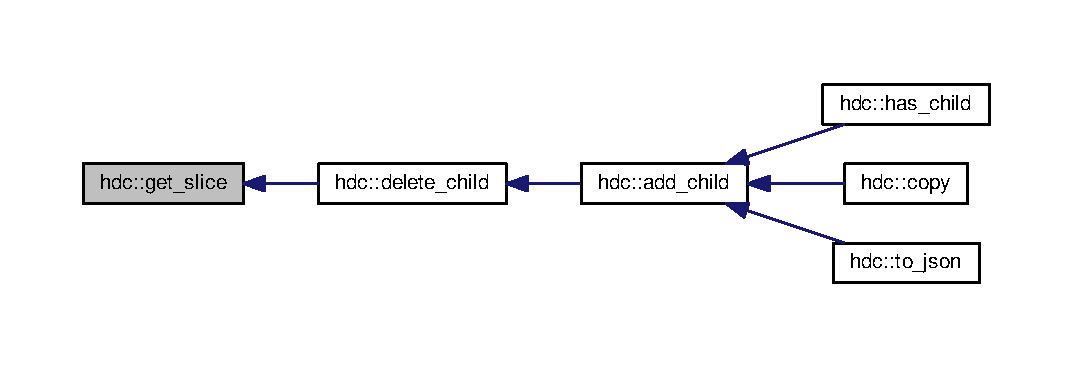
\includegraphics[width=350pt]{a00003_a580b1c84ebb50da63e2682ddceb6010a_icgraph}
\end{center}
\end{figure}


\index{hdc@{hdc}!get\+\_\+slice@{get\+\_\+slice}}
\index{get\+\_\+slice@{get\+\_\+slice}!hdc@{hdc}}
\subsubsection[{\texorpdfstring{get\+\_\+slice(size\+\_\+t i)}{get_slice(size_t i)}}]{\setlength{\rightskip}{0pt plus 5cm}{\bf hdc} $\ast$ hdc\+::get\+\_\+slice (
\begin{DoxyParamCaption}
\item[{size\+\_\+t}]{i}
\end{DoxyParamCaption}
)}\hypertarget{a00003_a1ef96265e222ef9acc07c151b20af8bf}{}\label{a00003_a1ef96265e222ef9acc07c151b20af8bf}


Returns i-\/th subnode if H\+D\+C\+\_\+\+L\+I\+ST is the type. 



Definition at line 208 of file hdc.\+cpp.


\begin{DoxyCode}
208                             \{
209     \textcolor{keywordflow}{if} (this->type == HDC\_LIST) \textcolor{keywordflow}{return} this->list\_elements->at(i);
210     \textcolor{keywordflow}{else} \textcolor{keywordflow}{return} \textcolor{keyword}{this}; \textcolor{comment}{// return this if not list}
211 \}
\end{DoxyCode}
\index{hdc@{hdc}!get\+\_\+type@{get\+\_\+type}}
\index{get\+\_\+type@{get\+\_\+type}!hdc@{hdc}}
\subsubsection[{\texorpdfstring{get\+\_\+type()}{get_type()}}]{\setlength{\rightskip}{0pt plus 5cm}uint8\+\_\+t hdc\+::get\+\_\+type (
\begin{DoxyParamCaption}
{}
\end{DoxyParamCaption}
)}\hypertarget{a00003_ac12e6d9074533304ea4d3eb08623d774}{}\label{a00003_ac12e6d9074533304ea4d3eb08623d774}


Appends given node as next available slice (similar to push\+\_\+back() method seen in C++ S\+TL containers). 



Definition at line 253 of file hdc.\+cpp.


\begin{DoxyCode}
254 \{
255     \textcolor{keywordflow}{return} this->type;
256 \}
\end{DoxyCode}
\index{hdc@{hdc}!get\+\_\+type\+\_\+str@{get\+\_\+type\+\_\+str}}
\index{get\+\_\+type\+\_\+str@{get\+\_\+type\+\_\+str}!hdc@{hdc}}
\subsubsection[{\texorpdfstring{get\+\_\+type\+\_\+str()}{get_type_str()}}]{\setlength{\rightskip}{0pt plus 5cm}string hdc\+::get\+\_\+type\+\_\+str (
\begin{DoxyParamCaption}
{}
\end{DoxyParamCaption}
)}\hypertarget{a00003_adb9061053ac1426deae825e364b340bc}{}\label{a00003_adb9061053ac1426deae825e364b340bc}


Returns void pointer to data. 



Definition at line 508 of file hdc.\+cpp.


\begin{DoxyCode}
508                          \{
509     \textcolor{keywordtype}{string} type\_str;
510     \textcolor{keywordflow}{if} (this->type == HDC\_EMPTY) type\_str = \textcolor{stringliteral}{"null"};
511     \textcolor{keywordflow}{else} \textcolor{keywordflow}{if} (this->type == HDC\_LIST || this->type == HDC\_STRUCT) type\_str = \textcolor{stringliteral}{"hdc"};
512     \textcolor{keywordflow}{else} \{
513         dynd::ndt::type dt;
514         \textcolor{keywordflow}{switch}(this->\hyperlink{a00003_a759758dd2b6b8986341753e94ad12252}{get\_ndim}()) \{
515             \textcolor{keywordflow}{case} 0:
516                 dt = this->data->at(0).get\_type();
517                 \textcolor{keywordflow}{break};
518             \textcolor{keywordflow}{case} 1:
519                 dt = this->data->at(0)(0).\hyperlink{a00003_ac12e6d9074533304ea4d3eb08623d774}{get\_type}();
520                 \textcolor{keywordflow}{break};
521             \textcolor{keywordflow}{case} 2:
522                 dt = this->data->at(0)(0,0).\hyperlink{a00003_ac12e6d9074533304ea4d3eb08623d774}{get\_type}();
523                 \textcolor{keywordflow}{break};
524             \textcolor{keywordflow}{case} 3:
525                 dt = this->data->at(0)(0,0,0).\hyperlink{a00003_ac12e6d9074533304ea4d3eb08623d774}{get\_type}();
526                 \textcolor{keywordflow}{break};
527             \textcolor{keywordflow}{case} 4:
528                 dt = this->data->at(0)(0,0,0,0).\hyperlink{a00003_ac12e6d9074533304ea4d3eb08623d774}{get\_type}();
529                 \textcolor{keywordflow}{break};
530             \textcolor{keywordflow}{case} 5:
531                 dt = this->data->at(0)(0,0,0,0,0).\hyperlink{a00003_ac12e6d9074533304ea4d3eb08623d774}{get\_type}();
532                 \textcolor{keywordflow}{break};
533             \textcolor{keywordflow}{default}: \textcolor{comment}{// Yes, I tried more.}
534                 cout << \textcolor{stringliteral}{"Error: unsupported number of dimensions."} << endl;
535                 \textcolor{keywordflow}{break};
536         \}
537         type\_str = dt.str();
538     \}
539     \textcolor{keywordflow}{return} type\_str;
540 \}
\end{DoxyCode}
\index{hdc@{hdc}!has\+\_\+child@{has\+\_\+child}}
\index{has\+\_\+child@{has\+\_\+child}!hdc@{hdc}}
\subsubsection[{\texorpdfstring{has\+\_\+child(string path)}{has_child(string path)}}]{\setlength{\rightskip}{0pt plus 5cm}bool hdc\+::has\+\_\+child (
\begin{DoxyParamCaption}
\item[{string}]{path}
\end{DoxyParamCaption}
)}\hypertarget{a00003_aee70cadad065fa643d8313e068734e59}{}\label{a00003_aee70cadad065fa643d8313e068734e59}


Returns i-\/th subnode if H\+D\+C\+\_\+\+L\+I\+ST is the type. 



Definition at line 51 of file hdc.\+cpp.


\begin{DoxyCode}
52 \{
53     \textcolor{keywordflow}{return} this->\hyperlink{a00003_aee70cadad065fa643d8313e068734e59}{has\_child}(split(path,\textcolor{charliteral}{'/'}));
54 \}
\end{DoxyCode}


Here is the call graph for this function\+:
\nopagebreak
\begin{figure}[H]
\begin{center}
\leavevmode
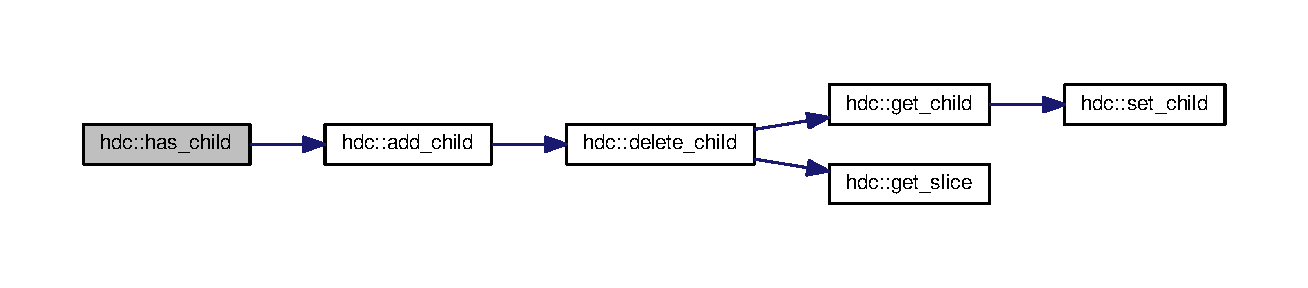
\includegraphics[width=350pt]{a00003_aee70cadad065fa643d8313e068734e59_cgraph}
\end{center}
\end{figure}


\index{hdc@{hdc}!is\+\_\+empty@{is\+\_\+empty}}
\index{is\+\_\+empty@{is\+\_\+empty}!hdc@{hdc}}
\subsubsection[{\texorpdfstring{is\+\_\+empty()}{is_empty()}}]{\setlength{\rightskip}{0pt plus 5cm}bool hdc\+::is\+\_\+empty (
\begin{DoxyParamCaption}
{}
\end{DoxyParamCaption}
)}\hypertarget{a00003_af1a86c27a06e02651f544947eb9b0cfb}{}\label{a00003_af1a86c27a06e02651f544947eb9b0cfb}


Sets H\+DC type of current node. 



Definition at line 322 of file hdc.\+cpp.


\begin{DoxyCode}
323 \{
324     \textcolor{keywordflow}{return} (this->type == HDC\_EMPTY);
325 \}
\end{DoxyCode}
\index{hdc@{hdc}!resize@{resize}}
\index{resize@{resize}!hdc@{hdc}}
\subsubsection[{\texorpdfstring{resize(hdc $\ast$h, int recursively=0)}{resize(hdc *h, int recursively=0)}}]{\setlength{\rightskip}{0pt plus 5cm}void hdc\+::resize (
\begin{DoxyParamCaption}
\item[{{\bf hdc} $\ast$}]{h, }
\item[{int}]{recursively = {\ttfamily 0}}
\end{DoxyParamCaption}
)}\hypertarget{a00003_ad782f111cf0c869166ed9f4ac51405a6}{}\label{a00003_ad782f111cf0c869166ed9f4ac51405a6}


Creates list with some data in nodes -\/ just for testing some ideas. 



Definition at line 423 of file hdc.\+cpp.


\begin{DoxyCode}
424 \{
425     \textcolor{keywordflow}{if} (this->type == HDC\_DYND) \{
426         \textcolor{keywordflow}{if} (!recursively) cout << \textcolor{stringliteral}{"Operation is yet not supported on the DYND node."} << endl;
427         \textcolor{keywordflow}{return};
428     \}
429     \textcolor{keywordflow}{else} \textcolor{keywordflow}{if} (this->type == HDC\_LIST) \{
430         \textcolor{keywordflow}{if} (!recursively) cout << \textcolor{stringliteral}{"Operation is yet not supported on the list node."} << endl;
431         \textcolor{keywordflow}{return};
432     \}
433     \textcolor{keywordflow}{else} \textcolor{keywordflow}{if} (this->type == HDC\_STRUCT) \{
434         \textcolor{keywordflow}{for} (\textcolor{keyword}{auto} it = h->children->begin(); it != h->children->end(); ++it) \{
435             \textcolor{keywordflow}{if} (!this->\hyperlink{a00003_aee70cadad065fa643d8313e068734e59}{has\_child}(it->first)) this->\hyperlink{a00003_a6ae2658ee66a5f4fb0d0d6535b36c5b2}{add\_child}(it->first,it->second->copy(0
      ));
436         \}
437         \textcolor{keywordflow}{return};
438     \}
439     \textcolor{keywordflow}{return};
440 \}
\end{DoxyCode}
\index{hdc@{hdc}!set\+\_\+child@{set\+\_\+child}}
\index{set\+\_\+child@{set\+\_\+child}!hdc@{hdc}}
\subsubsection[{\texorpdfstring{set\+\_\+child(string path, hdc $\ast$n)}{set_child(string path, hdc *n)}}]{\setlength{\rightskip}{0pt plus 5cm}void hdc\+::set\+\_\+child (
\begin{DoxyParamCaption}
\item[{string}]{path, }
\item[{{\bf hdc} $\ast$}]{n}
\end{DoxyParamCaption}
)}\hypertarget{a00003_acde60e58222d3b7d2b2a53b14289f500}{}\label{a00003_acde60e58222d3b7d2b2a53b14289f500}


Adds H\+DC subtree as child with given path. 

If neccessary, recursively creates subnodes. 

Definition at line 245 of file hdc.\+cpp.


\begin{DoxyCode}
245                                        \{
246     this->\hyperlink{a00003_acde60e58222d3b7d2b2a53b14289f500}{set\_child}(split(path,\textcolor{charliteral}{'/'}), n);
247     \textcolor{keywordflow}{return};
248 \}
\end{DoxyCode}


Here is the caller graph for this function\+:
\nopagebreak
\begin{figure}[H]
\begin{center}
\leavevmode
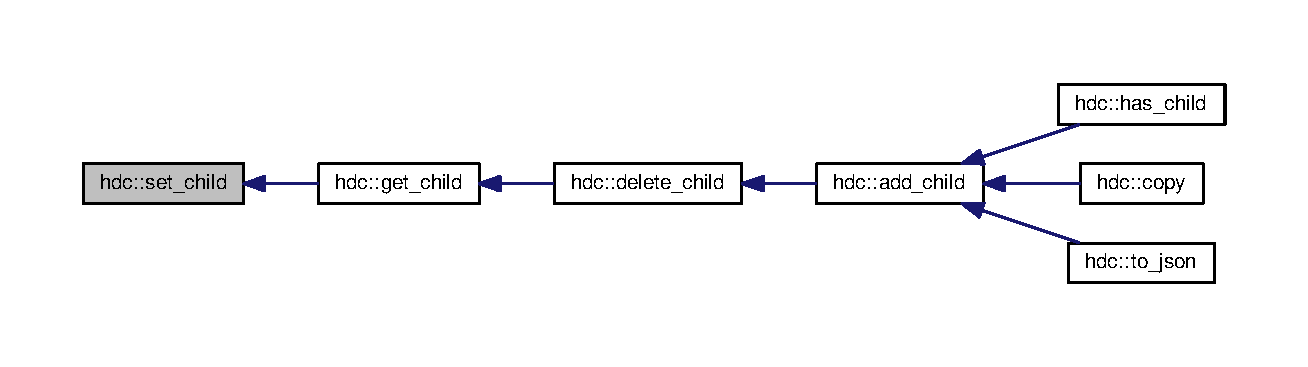
\includegraphics[width=350pt]{a00003_acde60e58222d3b7d2b2a53b14289f500_icgraph}
\end{center}
\end{figure}


\index{hdc@{hdc}!set\+\_\+data@{set\+\_\+data}}
\index{set\+\_\+data@{set\+\_\+data}!hdc@{hdc}}
\subsubsection[{\texorpdfstring{set\+\_\+data(vector$<$ T $>$ data)}{set_data(vector< T > data)}}]{\setlength{\rightskip}{0pt plus 5cm}template$<$typename T $>$ void hdc\+::set\+\_\+data (
\begin{DoxyParamCaption}
\item[{vector$<$ T $>$}]{data}
\end{DoxyParamCaption}
)\hspace{0.3cm}{\ttfamily [inline]}}\hypertarget{a00003_a120de413f9264db573e7c54aa49ae489}{}\label{a00003_a120de413f9264db573e7c54aa49ae489}


Returns true if subtree with given path with exists and false otherwise. 

Sets data to current node from vector$<$\+T$>$ data. This function is primarily designed for interoperability with Python 

Definition at line 48 of file hdc.\+hpp.


\begin{DoxyCode}
49     \{
50         \textcolor{keywordflow}{if} (this->children->size()) \{
51             cout << \textcolor{stringliteral}{"The node has already children set..."} << endl;
52             \textcolor{keywordflow}{return};
53         \}
54         \textcolor{comment}{//dynd::nd::array arr;}
55         \textcolor{comment}{//dynd::ndt::type dtype = dynd::ndt::make\_type<T>();}
56         \textcolor{comment}{//arr->data = (char*) data;}
57         dynd::nd::array arr = data;
58         cout << arr << endl;
59         \textcolor{keywordflow}{if} (this->data->size()) this->data->clear();
60         this->data->push\_back(arr);
61         \textcolor{comment}{//this->data = arr;}
62         this->type = HDC\_DYND;
63         \textcolor{keywordflow}{return};
64     \};
\end{DoxyCode}


Here is the caller graph for this function\+:
\nopagebreak
\begin{figure}[H]
\begin{center}
\leavevmode
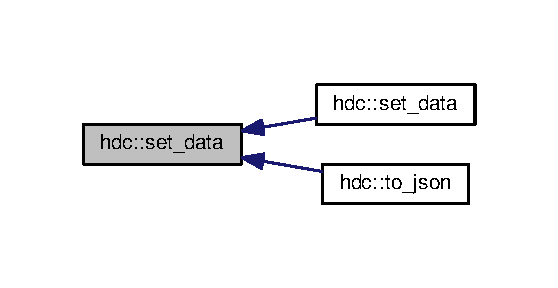
\includegraphics[width=268pt]{a00003_a120de413f9264db573e7c54aa49ae489_icgraph}
\end{center}
\end{figure}


\index{hdc@{hdc}!set\+\_\+data@{set\+\_\+data}}
\index{set\+\_\+data@{set\+\_\+data}!hdc@{hdc}}
\subsubsection[{\texorpdfstring{set\+\_\+data(string path, vector$<$ T $>$ data)}{set_data(string path, vector< T > data)}}]{\setlength{\rightskip}{0pt plus 5cm}template$<$typename T $>$ void hdc\+::set\+\_\+data (
\begin{DoxyParamCaption}
\item[{string}]{path, }
\item[{vector$<$ T $>$}]{data}
\end{DoxyParamCaption}
)\hspace{0.3cm}{\ttfamily [inline]}}\hypertarget{a00003_a9462ce2e878c8e978e38a9f71188973b}{}\label{a00003_a9462ce2e878c8e978e38a9f71188973b}


Sets data to node on given path from vector$<$\+T$>$ data. 

This function is primarily designed for interoperability with Python 

Definition at line 65 of file hdc.\+hpp.


\begin{DoxyCode}
66     \{
67         \textcolor{keywordflow}{if} (!this->\hyperlink{a00003_aee70cadad065fa643d8313e068734e59}{has\_child}(path)) \{
68             this->\hyperlink{a00003_a6ae2658ee66a5f4fb0d0d6535b36c5b2}{add\_child}(path, \textcolor{keyword}{new} \hyperlink{a00003}{hdc}());
69             cout << \textcolor{stringliteral}{"not found, adding..."} << endl;
70         \}
71         \hyperlink{a00003}{hdc}* t = this->\hyperlink{a00003_aafcd7c001cf4d3e2d61dbbf6efef6e08}{get\_child}(path);
72         t->\hyperlink{a00003_a120de413f9264db573e7c54aa49ae489}{set\_data}<T>(data);
73         \textcolor{keywordflow}{return};
74     \};
\end{DoxyCode}


Here is the call graph for this function\+:
\nopagebreak
\begin{figure}[H]
\begin{center}
\leavevmode
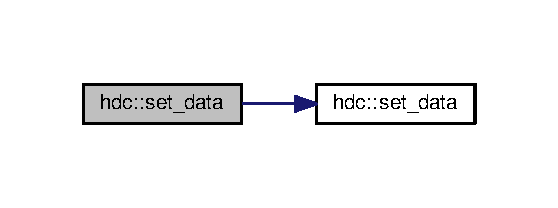
\includegraphics[width=268pt]{a00003_a9462ce2e878c8e978e38a9f71188973b_cgraph}
\end{center}
\end{figure}


\index{hdc@{hdc}!set\+\_\+data@{set\+\_\+data}}
\index{set\+\_\+data@{set\+\_\+data}!hdc@{hdc}}
\subsubsection[{\texorpdfstring{set\+\_\+data(int8\+\_\+t ndim, const long int $\ast$shape, void $\ast$data)}{set_data(int8_t ndim, const long int *shape, void *data)}}]{\setlength{\rightskip}{0pt plus 5cm}template$<$typename T $>$ void hdc\+::set\+\_\+data (
\begin{DoxyParamCaption}
\item[{int8\+\_\+t}]{ndim, }
\item[{const long int $\ast$}]{shape, }
\item[{void $\ast$}]{data}
\end{DoxyParamCaption}
)\hspace{0.3cm}{\ttfamily [inline]}}\hypertarget{a00003_a42e2debec93119c4e79ddefb49ff5c43}{}\label{a00003_a42e2debec93119c4e79ddefb49ff5c43}


Sets array data to current node. 



Definition at line 76 of file hdc.\+hpp.


\begin{DoxyCode}
77     \{
78         \textcolor{keywordflow}{if} (this->children->size()) \{
79             cout << \textcolor{stringliteral}{"The node has already children set..."} << endl;
80             \textcolor{keywordflow}{return};
81         \}
82         dynd::nd::array arr;
83         dynd::ndt::type dtype = dynd::ndt::make\_type<T>();
84         arr = dynd::nd::dtyped\_empty(ndim,shape,dtype);
85         arr->data = (\textcolor{keywordtype}{char}*) data;
86 \textcolor{comment}{//         arr.assign(data); // New versions of DyND}
87         cout << arr << endl;
88         \textcolor{keywordflow}{if} (this->data->size()) this->data->clear();
89         this->data->push\_back(arr);
90         \textcolor{comment}{//this->data = arr;}
91         this->type = HDC\_DYND;
92         \textcolor{keywordflow}{return};
93     \};
\end{DoxyCode}
\index{hdc@{hdc}!set\+\_\+data@{set\+\_\+data}}
\index{set\+\_\+data@{set\+\_\+data}!hdc@{hdc}}
\subsubsection[{\texorpdfstring{set\+\_\+data(string path, int8\+\_\+t ndim, const long int $\ast$shape, void $\ast$data)}{set_data(string path, int8_t ndim, const long int *shape, void *data)}}]{\setlength{\rightskip}{0pt plus 5cm}template$<$typename T $>$ void hdc\+::set\+\_\+data (
\begin{DoxyParamCaption}
\item[{string}]{path, }
\item[{int8\+\_\+t}]{ndim, }
\item[{const long int $\ast$}]{shape, }
\item[{void $\ast$}]{data}
\end{DoxyParamCaption}
)\hspace{0.3cm}{\ttfamily [inline]}}\hypertarget{a00003_a009b92dac161a40dc8e17231a4575c1a}{}\label{a00003_a009b92dac161a40dc8e17231a4575c1a}


Sets array data to node on given path. 



Definition at line 94 of file hdc.\+hpp.


\begin{DoxyCode}
95     \{
96         \textcolor{keywordflow}{if} (!this->\hyperlink{a00003_aee70cadad065fa643d8313e068734e59}{has\_child}(path)) \{
97             this->\hyperlink{a00003_a6ae2658ee66a5f4fb0d0d6535b36c5b2}{add\_child}(path, \textcolor{keyword}{new} \hyperlink{a00003}{hdc}());
98             cout << \textcolor{stringliteral}{"not found, adding..."} << endl;
99         \}
100         \hyperlink{a00003}{hdc}* t = this->\hyperlink{a00003_aafcd7c001cf4d3e2d61dbbf6efef6e08}{get\_child}(path);
101         t->\hyperlink{a00003_a120de413f9264db573e7c54aa49ae489}{set\_data}<T>(ndim,shape,data);
102         \textcolor{keywordflow}{return};
103     \};
\end{DoxyCode}


Here is the call graph for this function\+:
\nopagebreak
\begin{figure}[H]
\begin{center}
\leavevmode
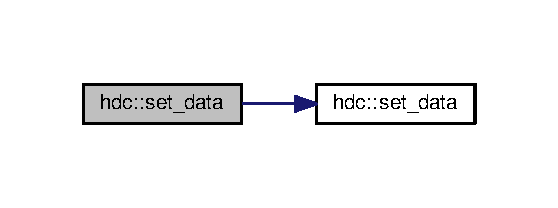
\includegraphics[width=268pt]{a00003_a009b92dac161a40dc8e17231a4575c1a_cgraph}
\end{center}
\end{figure}


\index{hdc@{hdc}!set\+\_\+data@{set\+\_\+data}}
\index{set\+\_\+data@{set\+\_\+data}!hdc@{hdc}}
\subsubsection[{\texorpdfstring{set\+\_\+data(\+T data)}{set_data(T data)}}]{\setlength{\rightskip}{0pt plus 5cm}template$<$typename T $>$ void hdc\+::set\+\_\+data (
\begin{DoxyParamCaption}
\item[{T}]{data}
\end{DoxyParamCaption}
)\hspace{0.3cm}{\ttfamily [inline]}}\hypertarget{a00003_a4465da11f7821ef4d405cd8805d77459}{}\label{a00003_a4465da11f7821ef4d405cd8805d77459}


Sets scalar data to current node. 



Definition at line 105 of file hdc.\+hpp.


\begin{DoxyCode}
106     \{
107         \textcolor{keywordflow}{if} (this->children->size()) \{
108             cout << \textcolor{stringliteral}{"The node has already children set..."} << endl;
109             \textcolor{keywordflow}{return};
110         \}
111         dynd::nd::array arr = data;
112         cout << arr << endl;
113         \textcolor{keywordflow}{if} (this->data->size()) this->data->clear();
114         this->data->push\_back(arr);
115         \textcolor{comment}{//this->data = arr;}
116         this->type = HDC\_DYND;
117         \textcolor{keywordflow}{return};
118     \};
\end{DoxyCode}
\index{hdc@{hdc}!set\+\_\+data@{set\+\_\+data}}
\index{set\+\_\+data@{set\+\_\+data}!hdc@{hdc}}
\subsubsection[{\texorpdfstring{set\+\_\+data(string path, T data)}{set_data(string path, T data)}}]{\setlength{\rightskip}{0pt plus 5cm}template$<$typename T $>$ void hdc\+::set\+\_\+data (
\begin{DoxyParamCaption}
\item[{string}]{path, }
\item[{T}]{data}
\end{DoxyParamCaption}
)\hspace{0.3cm}{\ttfamily [inline]}}\hypertarget{a00003_a5a15d6128e566f802263c3fbf69a1d49}{}\label{a00003_a5a15d6128e566f802263c3fbf69a1d49}


Sets scalar data to node on given path. 



Definition at line 119 of file hdc.\+hpp.


\begin{DoxyCode}
120     \{
121         \textcolor{keywordflow}{if} (!this->\hyperlink{a00003_aee70cadad065fa643d8313e068734e59}{has\_child}(path)) \{
122             this->\hyperlink{a00003_a6ae2658ee66a5f4fb0d0d6535b36c5b2}{add\_child}(path, \textcolor{keyword}{new} \hyperlink{a00003}{hdc}());
123             cout << \textcolor{stringliteral}{"not found, adding..."} << endl;
124         \}
125         \hyperlink{a00003}{hdc}* t = this->\hyperlink{a00003_aafcd7c001cf4d3e2d61dbbf6efef6e08}{get\_child}(path);
126         t->\hyperlink{a00003_a120de413f9264db573e7c54aa49ae489}{set\_data}(data);
127         \textcolor{keywordflow}{return};
128     \};
\end{DoxyCode}


Here is the call graph for this function\+:
\nopagebreak
\begin{figure}[H]
\begin{center}
\leavevmode
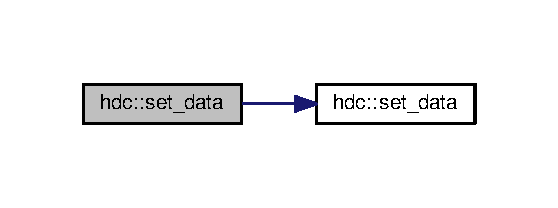
\includegraphics[width=268pt]{a00003_a5a15d6128e566f802263c3fbf69a1d49_cgraph}
\end{center}
\end{figure}


\index{hdc@{hdc}!set\+\_\+list@{set\+\_\+list}}
\index{set\+\_\+list@{set\+\_\+list}!hdc@{hdc}}
\subsubsection[{\texorpdfstring{set\+\_\+list(vector$<$ hdc $\ast$ $>$ $\ast$list)}{set_list(vector< hdc * > *list)}}]{\setlength{\rightskip}{0pt plus 5cm}void hdc\+::set\+\_\+list (
\begin{DoxyParamCaption}
\item[{vector$<$ {\bf hdc} $\ast$ $>$ $\ast$}]{list}
\end{DoxyParamCaption}
)}\hypertarget{a00003_ae3cf31bad48437a48ad1291e2db99873}{}\label{a00003_ae3cf31bad48437a48ad1291e2db99873}


Sets Dy\+ND object to current node. 



Definition at line 107 of file hdc.\+cpp.


\begin{DoxyCode}
107                                      \{
108     \textcolor{keywordflow}{if} (this->type != HDC\_EMPTY) \{
109         cout << \textcolor{stringliteral}{"Cannot add list to a non-list node."} << endl;
110     \}
111     this->list\_elements = list;
112     \textcolor{keywordflow}{return};
113 \}
\end{DoxyCode}
\index{hdc@{hdc}!set\+\_\+slice@{set\+\_\+slice}}
\index{set\+\_\+slice@{set\+\_\+slice}!hdc@{hdc}}
\subsubsection[{\texorpdfstring{set\+\_\+slice(size\+\_\+t i, hdc $\ast$h)}{set_slice(size_t i, hdc *h)}}]{\setlength{\rightskip}{0pt plus 5cm}void hdc\+::set\+\_\+slice (
\begin{DoxyParamCaption}
\item[{size\+\_\+t}]{i, }
\item[{{\bf hdc} $\ast$}]{h}
\end{DoxyParamCaption}
)}\hypertarget{a00003_a3d4c2ba09c79e2dfbe7be7bd59bd811e}{}\label{a00003_a3d4c2ba09c79e2dfbe7be7bd59bd811e}


Returns copy of current object. 



Definition at line 478 of file hdc.\+cpp.


\begin{DoxyCode}
479 \{
480     cout << \textcolor{stringliteral}{"Setting slice "} << i << endl;
481     \textcolor{keywordflow}{if} (this->type == HDC\_LIST) \{
482         \textcolor{keywordflow}{if} (i < this->list\_elements->size()) this->list\_elements->at(i) = h;
483         \textcolor{keywordflow}{else} \textcolor{keywordflow}{if} (i == this->list\_elements->size()) this->\hyperlink{a00003_aaffff0cd041746fd45a2d2c67d73ce75}{append\_slice}(h);
484         \textcolor{keywordflow}{else} cout << \textcolor{stringliteral}{"Error in set\_slice(): Array too small."} << endl;
485     \} \textcolor{keywordflow}{else} cout << \textcolor{stringliteral}{"Error in set\_slice(): Wrong type to call set\_slice."} << endl;
486     \textcolor{keywordflow}{return};
487 \}
\end{DoxyCode}


Here is the caller graph for this function\+:
\nopagebreak
\begin{figure}[H]
\begin{center}
\leavevmode
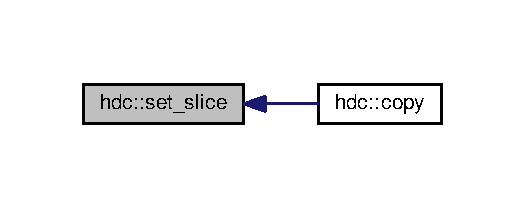
\includegraphics[width=252pt]{a00003_a3d4c2ba09c79e2dfbe7be7bd59bd811e_icgraph}
\end{center}
\end{figure}


\index{hdc@{hdc}!set\+\_\+type@{set\+\_\+type}}
\index{set\+\_\+type@{set\+\_\+type}!hdc@{hdc}}
\subsubsection[{\texorpdfstring{set\+\_\+type(uint8\+\_\+t i)}{set_type(uint8_t i)}}]{\setlength{\rightskip}{0pt plus 5cm}void hdc\+::set\+\_\+type (
\begin{DoxyParamCaption}
\item[{uint8\+\_\+t}]{i}
\end{DoxyParamCaption}
)}\hypertarget{a00003_a6d1d1064db92be176775481eb6ca9fd3}{}\label{a00003_a6d1d1064db92be176775481eb6ca9fd3}


Returns type of current node. 



Definition at line 258 of file hdc.\+cpp.


\begin{DoxyCode}
258                             \{
259     \textcolor{comment}{// More to be added here later}
260     this->type = i;
261     \textcolor{keywordflow}{if} (i == HDC\_LIST && this->list\_elements == \textcolor{keyword}{nullptr}) this->list\_elements = \textcolor{keyword}{new} vector<hdc*>;
262     \textcolor{keywordflow}{return};
263 \}
\end{DoxyCode}


Here is the caller graph for this function\+:
\nopagebreak
\begin{figure}[H]
\begin{center}
\leavevmode
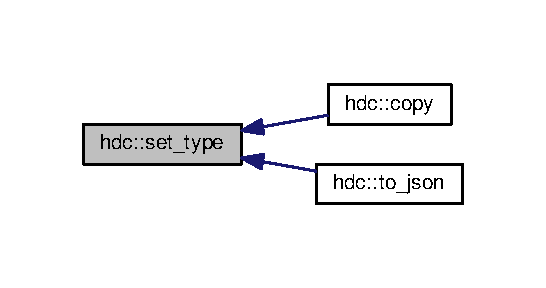
\includegraphics[width=262pt]{a00003_a6d1d1064db92be176775481eb6ca9fd3_icgraph}
\end{center}
\end{figure}


\index{hdc@{hdc}!to\+\_\+json@{to\+\_\+json}}
\index{to\+\_\+json@{to\+\_\+json}!hdc@{hdc}}
\subsubsection[{\texorpdfstring{to\+\_\+json(string filename, int mode=0)}{to_json(string filename, int mode=0)}}]{\setlength{\rightskip}{0pt plus 5cm}void hdc\+::to\+\_\+json (
\begin{DoxyParamCaption}
\item[{string}]{filename, }
\item[{int}]{mode = {\ttfamily 0}}
\end{DoxyParamCaption}
)}\hypertarget{a00003_af7684e94ec717ae6e9de1ba1f0e6bff0}{}\label{a00003_af7684e94ec717ae6e9de1ba1f0e6bff0}


Returns pointer to self. 



Definition at line 556 of file hdc.\+cpp.


\begin{DoxyCode}
557 \{
558     cout << \textcolor{stringliteral}{"Saving output JSON to "} << filename << endl;
559     ofstream json\_file;
560     json\_file.open(filename.c\_str());
561     \textcolor{comment}{// json\_file << this->to\_json();}
562     \textcolor{comment}{// get rid of quotes produced by writing dynd::nd::array.as<string>}
563     \textcolor{comment}{// see https://www.youtube.com/watch?v=SiUz\_akTmcY for details...}
564     stringstream tmp;
565     tmp << this->\hyperlink{a00003_af7684e94ec717ae6e9de1ba1f0e6bff0}{to\_json}(mode);
566     \textcolor{keywordtype}{string} tmp\_str = tmp.str();
567     \textcolor{keywordtype}{string} la(\textcolor{stringliteral}{"["}); \textcolor{comment}{// left after}
568     \textcolor{keywordtype}{string} lb(\textcolor{stringliteral}{"\(\backslash\)"["}); \textcolor{comment}{// left before}
569     replace\_all(tmp\_str,lb,la);
570     \textcolor{keywordtype}{string} ra(\textcolor{stringliteral}{"]"}); \textcolor{comment}{// right after}
571     \textcolor{keywordtype}{string} rb(\textcolor{stringliteral}{"]\(\backslash\)""}); \textcolor{comment}{// right before}
572     replace\_all(tmp\_str,rb,ra);
573     cout << tmp\_str;
574     json\_file << tmp\_str;
575     \textcolor{comment}{// end of quotes removal}
576     json\_file.close();
577 
578     \textcolor{keywordflow}{return};
579 \}
\end{DoxyCode}


Here is the call graph for this function\+:
\nopagebreak
\begin{figure}[H]
\begin{center}
\leavevmode
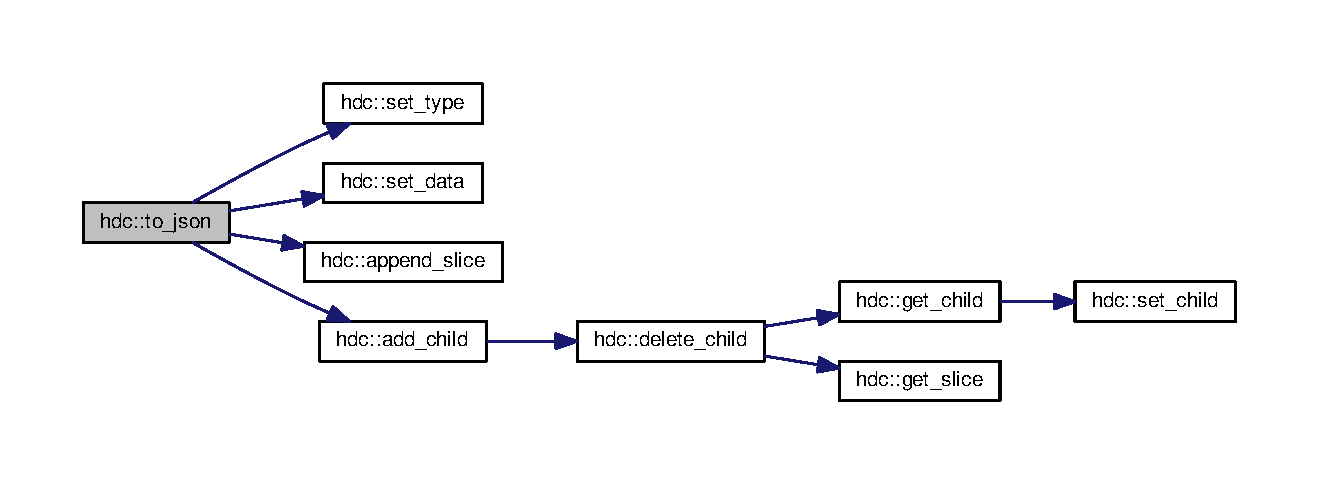
\includegraphics[width=350pt]{a00003_af7684e94ec717ae6e9de1ba1f0e6bff0_cgraph}
\end{center}
\end{figure}


\index{hdc@{hdc}!to\+\_\+json@{to\+\_\+json}}
\index{to\+\_\+json@{to\+\_\+json}!hdc@{hdc}}
\subsubsection[{\texorpdfstring{to\+\_\+json(int mode=0)}{to_json(int mode=0)}}]{\setlength{\rightskip}{0pt plus 5cm}Json\+::\+Value hdc\+::to\+\_\+json (
\begin{DoxyParamCaption}
\item[{int}]{mode = {\ttfamily 0}}
\end{DoxyParamCaption}
)}\hypertarget{a00003_a801f7f1bd6c145b0fef673b99b0724d2}{}\label{a00003_a801f7f1bd6c145b0fef673b99b0724d2}


Serialization to J\+S\+ON file. 



Definition at line 347 of file hdc.\+cpp.


\begin{DoxyCode}
347                                \{
348     Json::Value root;
349     \textcolor{keywordflow}{if} (mode == 0) \{
350         \textcolor{keywordflow}{if} (this->type == HDC\_DYND) \{
351             root = dynd::format\_json(this->data->at(0)).as<string>();        
352         \}
353         \textcolor{keywordflow}{else} \textcolor{keywordflow}{if} (this->type == HDC\_STRUCT) \{
354             \textcolor{keywordflow}{for} (\textcolor{keyword}{auto} it = this->children->begin(); it != this->children->end(); it++) \{
355                 Json::Value child;
356                 child[it->first] = it->second->to\_json(mode);
357                 it->second;
358                 \textcolor{comment}{//root.append(child);}
359                 root[it->first] = it->second->to\_json(mode);
360             \}
361         \}
362         \textcolor{keywordflow}{else} \textcolor{keywordflow}{if} (this->type == HDC\_LIST) \{
363             Json::Value elements;
364             \textcolor{keywordflow}{for} (\textcolor{keywordtype}{long} i=0;i<this->list\_elements->size();i++) root.append(this->list\_elements->at(i)->
      to\_json(mode));        
365         \}
366     \}
367     \textcolor{keywordflow}{else} \textcolor{keywordflow}{if} (mode == 1) \{
368             \textcolor{keywordflow}{if} (this->type == HDC\_DYND) \{
369             dynd::ndt::type dt;
370             \textcolor{keywordflow}{switch}(this->\hyperlink{a00003_a759758dd2b6b8986341753e94ad12252}{get\_ndim}()) \{ \textcolor{comment}{// I really don't want to spend several hours by digging
       into dynd sources, sorry.}
371                 \textcolor{keywordflow}{case} 0:
372                     dt = this->data->at(0).get\_type();
373                     \textcolor{keywordflow}{break};
374                 \textcolor{keywordflow}{case} 1:
375                     dt = this->data->at(0)(0).\hyperlink{a00003_ac12e6d9074533304ea4d3eb08623d774}{get\_type}();
376                     \textcolor{keywordflow}{break};
377                 \textcolor{keywordflow}{case} 2:
378                     dt = this->data->at(0)(0,0).\hyperlink{a00003_ac12e6d9074533304ea4d3eb08623d774}{get\_type}();
379                     \textcolor{keywordflow}{break};
380                 \textcolor{keywordflow}{case} 3:
381                     dt = this->data->at(0)(0,0,0).\hyperlink{a00003_ac12e6d9074533304ea4d3eb08623d774}{get\_type}();
382                     \textcolor{keywordflow}{break};
383                 \textcolor{keywordflow}{case} 4:
384                     dt = this->data->at(0)(0,0,0,0).\hyperlink{a00003_ac12e6d9074533304ea4d3eb08623d774}{get\_type}();
385                     \textcolor{keywordflow}{break};
386                 \textcolor{keywordflow}{case} 5:
387                     dt = this->data->at(0)(0,0,0,0,0).\hyperlink{a00003_ac12e6d9074533304ea4d3eb08623d774}{get\_type}();
388                     \textcolor{keywordflow}{break};
389                 \textcolor{keywordflow}{default}: \textcolor{comment}{// Yes, I tried more.}
390                     cout << \textcolor{stringliteral}{"Error: unsupported number of dimensions."} << endl;
391                     \textcolor{keywordflow}{break};
392             \}
393             root[\textcolor{stringliteral}{"dtype"}] = dt.str();
394             root[\textcolor{stringliteral}{"data"}] = dynd::format\_json(this->data->at(0)).as<string>();        
395         \}
396         \textcolor{keywordflow}{else} \textcolor{keywordflow}{if} (this->type == HDC\_STRUCT) \{
397 \textcolor{comment}{//             Json::Value children;}
398             \textcolor{keywordflow}{for} (\textcolor{keyword}{auto} it = this->children->begin(); it != this->children->end(); it++) \{
399                 Json::Value child;
400                 child[it->first] = it->second->to\_json(mode);
401                 it->second;
402                 root.append(child);
403 \textcolor{comment}{//                 children[it->first] = it->second->to\_json(mode);}
404             \}
405 \textcolor{comment}{//             root["dtype"] = "hdc\_struct";}
406 \textcolor{comment}{//             root["data"] = children;}
407         \}
408         \textcolor{keywordflow}{else} \textcolor{keywordflow}{if} (this->type == HDC\_LIST) \{
409             Json::Value elements;
410 \textcolor{comment}{//             for (long i=0;i<this->list\_elements->size();i++)
       elements.append(this->list\_elements->at(i)->to\_json(mode));}
411 \textcolor{comment}{//             root["dtype"] = "hdc\_list";}
412 \textcolor{comment}{//             root["data"] = elements;}
413             \textcolor{keywordflow}{for} (\textcolor{keywordtype}{long} i=0;i<this->list\_elements->size();i++) root.append(this->list\_elements->at(i)->
      to\_json(mode));
414 
415         \}
416 \textcolor{comment}{//         else if (this->type == HDC\_EMPTY) \{}
417 \textcolor{comment}{//             root["dtype"] = "hdc\_empty";}
418 \textcolor{comment}{//         \}}
419     \}
420     \textcolor{keywordflow}{return} root;
421 \}
\end{DoxyCode}


The documentation for this class was generated from the following files\+:\begin{DoxyCompactItemize}
\item 
/home/david/projects/hdc\+\_\+new/inc/hdc.\+hpp\item 
/home/david/projects/hdc\+\_\+new/src/hdc.\+cpp\end{DoxyCompactItemize}

\hypertarget{a00004}{}\section{hdc\+\_\+fortran\+:\+:hdc\+\_\+new\+\_\+empty Interface Reference}
\label{a00004}\index{hdc\+\_\+fortran\+::hdc\+\_\+new\+\_\+empty@{hdc\+\_\+fortran\+::hdc\+\_\+new\+\_\+empty}}


\subsection{Detailed Description}


Definition at line 20 of file hdc\+\_\+fortran.\+f90.



The documentation for this interface was generated from the following file\+:\begin{DoxyCompactItemize}
\item 
/home/david/projects/hdc\+\_\+new/src/hdc\+\_\+fortran.\+f90\end{DoxyCompactItemize}

\hypertarget{a00005}{}\section{test\+\_\+hdc\+\_\+pybind11.\+H\+D\+C\+\_\+T Class Reference}
\label{a00005}\index{test\+\_\+hdc\+\_\+pybind11.\+H\+D\+C\+\_\+T@{test\+\_\+hdc\+\_\+pybind11.\+H\+D\+C\+\_\+T}}


Inheritance diagram for test\+\_\+hdc\+\_\+pybind11.\+H\+D\+C\+\_\+T\+:
\nopagebreak
\begin{figure}[H]
\begin{center}
\leavevmode
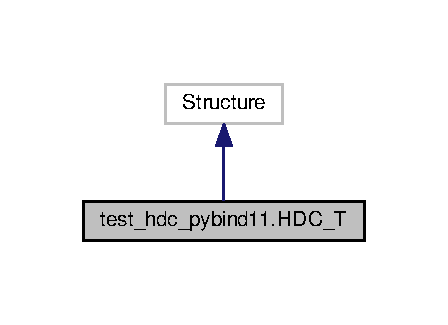
\includegraphics[width=215pt]{a00045}
\end{center}
\end{figure}


Collaboration diagram for test\+\_\+hdc\+\_\+pybind11.\+H\+D\+C\+\_\+T\+:
\nopagebreak
\begin{figure}[H]
\begin{center}
\leavevmode
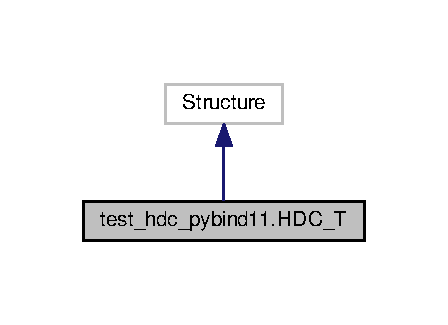
\includegraphics[width=215pt]{a00046}
\end{center}
\end{figure}


\subsection{Detailed Description}


Definition at line 16 of file test\+\_\+hdc\+\_\+pybind11.\+py.



The documentation for this class was generated from the following file\+:\begin{DoxyCompactItemize}
\item 
/home/david/projects/hdc\+\_\+new/src/tests/test\+\_\+hdc\+\_\+pybind11.\+py\end{DoxyCompactItemize}

\hypertarget{a00006}{}\section{test\+\_\+hdc\+\_\+py\+\_\+c.\+H\+D\+C\+\_\+T Class Reference}
\label{a00006}\index{test\+\_\+hdc\+\_\+py\+\_\+c.\+H\+D\+C\+\_\+T@{test\+\_\+hdc\+\_\+py\+\_\+c.\+H\+D\+C\+\_\+T}}


Inheritance diagram for test\+\_\+hdc\+\_\+py\+\_\+c.\+H\+D\+C\+\_\+T\+:
\nopagebreak
\begin{figure}[H]
\begin{center}
\leavevmode
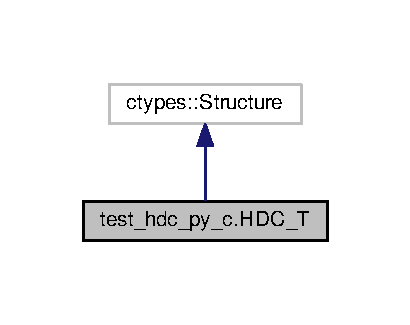
\includegraphics[width=197pt]{a00043}
\end{center}
\end{figure}


Collaboration diagram for test\+\_\+hdc\+\_\+py\+\_\+c.\+H\+D\+C\+\_\+T\+:
\nopagebreak
\begin{figure}[H]
\begin{center}
\leavevmode
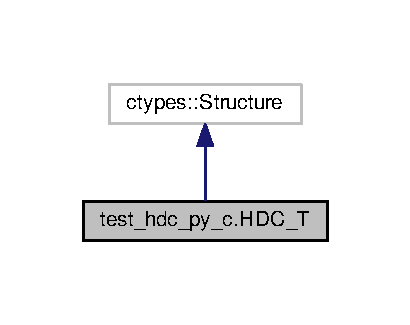
\includegraphics[width=197pt]{a00044}
\end{center}
\end{figure}


\subsection{Detailed Description}


Definition at line 7 of file test\+\_\+hdc\+\_\+py\+\_\+c.\+py.



The documentation for this class was generated from the following file\+:\begin{DoxyCompactItemize}
\item 
/home/david/projects/hdc\+\_\+new/src/tests/test\+\_\+hdc\+\_\+py\+\_\+c.\+py\end{DoxyCompactItemize}

\hypertarget{a00007}{}\section{hdc\+\_\+t Struct Reference}
\label{a00007}\index{hdc\+\_\+t@{hdc\+\_\+t}}
\subsection*{Public Attributes}
\begin{DoxyCompactItemize}
\item 
void $\ast$ {\bfseries obj}\hypertarget{a00007_af998aa25515681a151a201355fc9e108}{}\label{a00007_af998aa25515681a151a201355fc9e108}

\end{DoxyCompactItemize}


\subsection{Detailed Description}


Definition at line 5 of file hdc.\+cpp.



The documentation for this struct was generated from the following files\+:\begin{DoxyCompactItemize}
\item 
/home/david/projects/hdc\+\_\+new/src/hdc.\+cpp\item 
/home/david/projects/hdc\+\_\+new/src/hdc\+\_\+c.\+cpp\item 
/home/david/projects/hdc\+\_\+new/src/hdc\+\_\+python.\+cpp\end{DoxyCompactItemize}

\hypertarget{a00008}{}\section{types\+:\+:hdc\+\_\+t Type Reference}
\label{a00008}\index{types\+::hdc\+\_\+t@{types\+::hdc\+\_\+t}}
\subsection*{Public Attributes}
\begin{DoxyCompactItemize}
\item 
type(c\+\_\+ptr) {\bfseries obj}\hypertarget{a00008_a3d68238bd16580d6c092d8bafc20f1c7}{}\label{a00008_a3d68238bd16580d6c092d8bafc20f1c7}

\end{DoxyCompactItemize}


\subsection{Detailed Description}


Definition at line 4 of file hdc\+\_\+fortran.\+f90.



The documentation for this type was generated from the following file\+:\begin{DoxyCompactItemize}
\item 
/home/david/projects/hdc\+\_\+new/src/hdc\+\_\+fortran.\+f90\end{DoxyCompactItemize}

\hypertarget{a00009}{}\section{identity$<$ T $>$ Struct Template Reference}
\label{a00009}\index{identity$<$ T $>$@{identity$<$ T $>$}}
\subsection*{Public Types}
\begin{DoxyCompactItemize}
\item 
typedef T {\bfseries type}\hypertarget{a00009_af1d3cc50c66b9e147900b63d85cdd841}{}\label{a00009_af1d3cc50c66b9e147900b63d85cdd841}

\end{DoxyCompactItemize}


\subsection{Detailed Description}
\subsubsection*{template$<$typename T$>$\\*
struct identity$<$ T $>$}



Definition at line 32 of file hdc.\+hpp.



The documentation for this struct was generated from the following file\+:\begin{DoxyCompactItemize}
\item 
/home/david/projects/hdc\+\_\+new/inc/hdc.\+hpp\end{DoxyCompactItemize}

%--- End generated contents ---

% Index
\backmatter
\newpage
\phantomsection
\clearemptydoublepage
\addcontentsline{toc}{chapter}{Index}
\printindex

\end{document}
